\documentclass{article}
\usepackage{amsmath, amssymb, amsthm}
\usepackage{graphicx} % For adding images
\usepackage{float}
\graphicspath{{images/}}

% Customization
\newtheorem{definition}{Definition}
\theoremstyle{definition}
\newtheorem{example}{Example}[section]
%GEOMETRY
\usepackage[letterpaper, top=1.0in, bottom=1.0in, left=1.0in, right=1.0in, heightrounded]{geometry}

%line height
\renewcommand{\baselinestretch}{1.15}

%parskip and parindent
\setlength{\parindent}{0pt}
\setlength{\parskip}{0.8em}

\begin{document}
%TODO: add title page and tables of contents

\section{Chapter 1}

\subsection*{1.0}

There are 6 main issues we will focus on in economics:
\begin{itemize}
    \item \begin{definition}Productivity Growth\end{definition}
    Productivity is measured by ${Productivity=Output/Worker}$\\
    Incentives lead to productivity growth.
    \item \begin{definition} Population Growth\end{definition}
    Canada is open to immigrants, we have a low birth rate compared to past generations.
    No population growth leads to less workers, meaning workers must work harder.
    There are benefits and costs of having children.
    \item \begin{definition}Climate Change\end{definition}
    Cities in Canada and moving towards bodies of waters. Risk of submersion.
    Need to think about city design and allocation of people and resources.
    \begin{example}
        Farmers' harvests are affected by climate change. Impacts their income.
    \end{example}
    Economic impact of climate change is a big issue.
    \item \begin{definition}Technological Change\end{definition}
    Changing many industries, including education.
    Automation, job losses but also new job markets.
    Presently, might technological change may seem to be bad news but the future brings changes.
    \item \begin{definition}Protectionism\end{definition}
    Has been, unfortunately, on the rise over 20-40 years.
    Opposed to trade or comes with conditions.
    Countries have decided to tie trades to labour and climate conditions and standards.
    Free trade resists protectionism.
    \item \begin{definition}Inequality\end{definition}
    Highly undesirable, unless you are at the top of the distribution.
    Not within your control.
    Income inequality is problematic but has a deeper understanding. There is a difference between unfair and inequal.
    Need to analyze individual potential.
\end{itemize}

\subsection{}
\begin{definition}
    Economics is a social science that studies how we allocate limited resources
    to satisfy unlimited wants.
\end{definition}
\begin{definition}
    Social science is the study of people.
\end{definition}
Is the allocation of resources fair? just? efficient?
By resources we mean:
\begin{itemize}
    \item Land (T)
    \item Labour (L)
    \item Capital (K) 
\end{itemize}
Note: Money is not a resource, it is a means of making exchange easier.
With Land, Labour or Capital you could make use of them on a island alone.

These resources are limited or scarce but \textbf{our wants are unlimited}. Even billionaires give away their money for their wants.
Scarcity $\rightarrow$ Choice.
\begin{figure}[h!]
    \begin{minipage}{\textwidth}
        \centering
        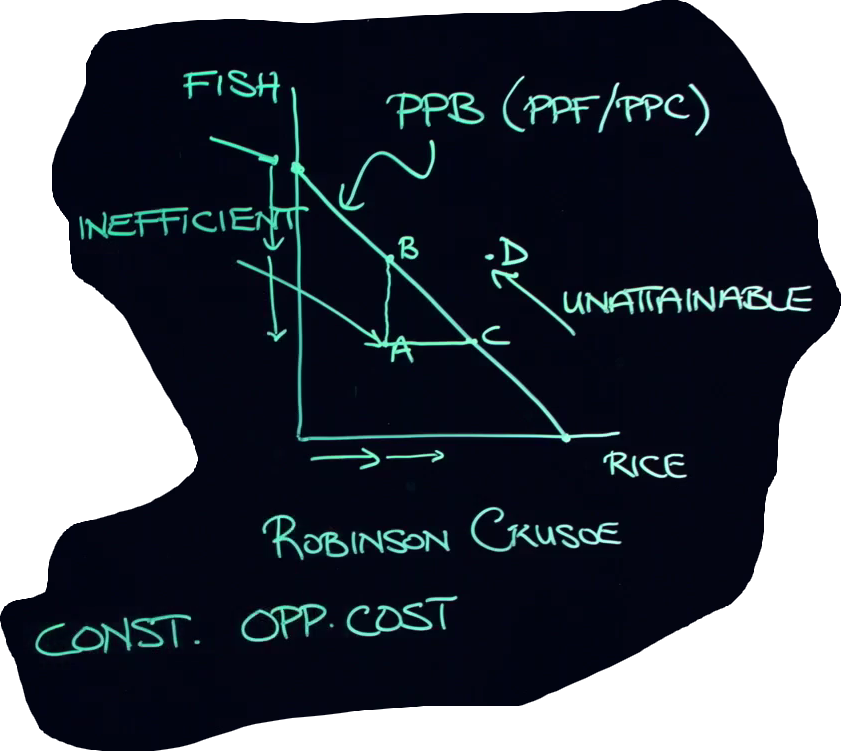
\includegraphics[width=0.5\textwidth]{RobinsonConstant.png}
        \caption[Constant Opportunity Cost]{Robinson Crusoe\footnote[1]{Story of a life of comfort to a solitary existence on a deserted island}'s Constant Opportunity Cost}
    \end{minipage}
\end{figure}
\begin{center}
\end{center}
Naturally we try to equalize the values of rice and fish (EQUITY).
If we used all of Crusoe's resources we would get a linear line (PPB/PPF/PPC meaning Production Possibility). Say that point A is below the line. This means it is potential with his resources but we say it is \textbf{inefficient}.
Same with point B and C but they maximize his resources. Point D is above the line and is \textbf{unattainable}, meaning he cannot achieve it.

\begin{definition}
    Opportunity Cost is the value of the next best alternative forgone.
    \begin{example}
    If Crusoe has maximized his use of resources, to acquire more rice, Crusoe must give up some fish.
    The cost is constant in this example.
    \end{example}
    Note: In real life, a constant opportunity cost is generally not realistic.
\end{definition}
Imagine Crusoe's opportunity cost is no longer constant but increasing.
The graph of his resources would be a slope.\\
\begin{figure}[h!]
    \centering
    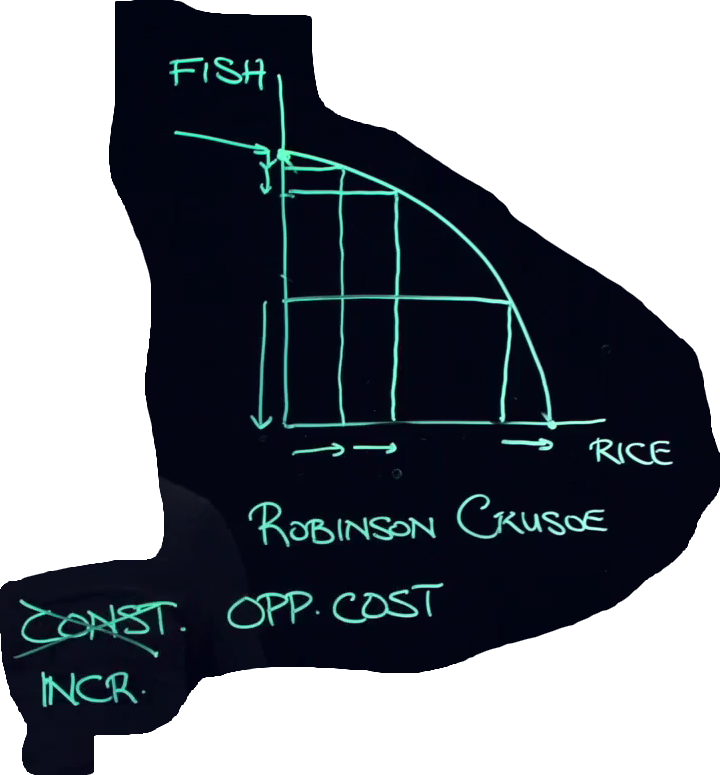
\includegraphics[width=0.5\textwidth]{RobinsonIncreasing.png}
    \caption{Robinson Crusoe's Increasing Opportunity Cost}
\end{figure}
Crusoe is able to give up the inefficent methods of obtaining fish/rice for the other initially.
To obtain more and more of the other, he must give up more and more of the other. This is the law of increasing opportunity cost.

\subsection{}

\begin{definition}
    Market Economy is an economy where resources are allocated through the decentralized decisions of many firms and households as they interact in markets for goods and services.
    The economy is characterized by being self-organizing and efficient.
    We assume that the agents of the market are self-interested and incentivized.
\end{definition}

The three agents are individuals, firms and government and are all interested in maximizing something.
Individuals maximize utility (happiness), firms maximize profit and government maximizes social welfare (in an ideal world).

\begin{definition}
    Incentives are rewards or penalties that motivate behaviour.
\end{definition}

\begin{definition}
    Free Trade is the policy of not discriminating against imports from other countries and relying on the market to allocate resources.
\end{definition}

\begin{definition}
    Protectionism is the policy of protecting domestic industries against foreign competition by imposing tariffs, quotas and other trade barriers.
\end{definition}

\begin{example}
    Let us focus on two agents: individuals and firms and three markets: goods (tangible) and services (intangible), financial and factor.
    \begin{figure}[h!]
        \centering
        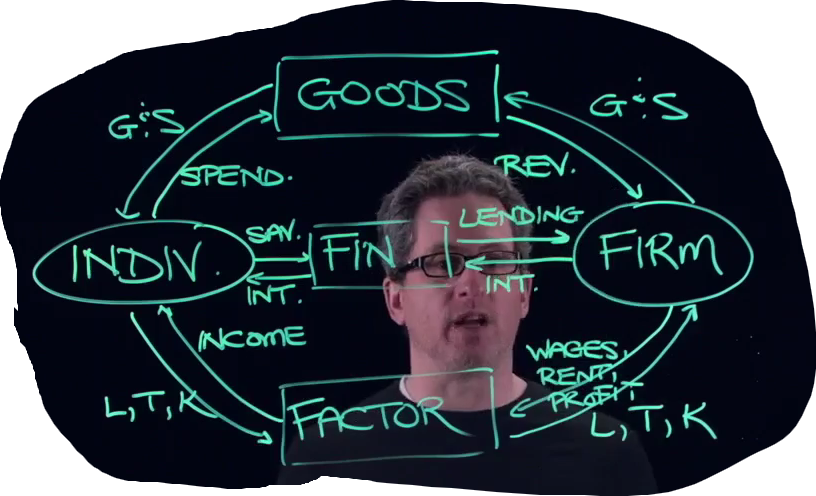
\includegraphics[width=0.5\textwidth]{CircularFlowOfIncomeAndExpenditure.png}
        \caption{Circular Flow of Income and Expenditure}
    \end{figure}
    Firms provide goods and services to the goods and services market and expect revenue.
    The factor market provides firms with resources (T, L and K) and expect wages, rent and profit.
    Individuals receive income (wages, rent and profit) from the factor market and provide resources (T, L and K).
    Individuals spend their income on goods and services in the goods and services market.
    Individuals save their income in the financial market and expect interest.
    Firms lend from the financial market and the market expects interest.

\end{example}

\subsection{}
Market Economy is generally the most efficient way to allocate resources. However, there are some limitations to the market economy.

Alternatives to the Market Economy:
\begin{itemize}
    \item Traditional Economy: Resources are allocated based on inheritance and custom. \begin{quote}"We've always done it that way."\end{quote}
    \item Command Economy: Resources are allocated by a centralized authority.
    \item Mixed Economy: Resources are allocated by a combination of market, tradition and command.
\end{itemize}

Gouvernment's Role in the Market Economy, correcting where the market fails:
\begin{itemize}
    \item Institutions
    \item Legal System
    \item Courts
    \item Justice
    \item Public Goods - Goods that cannot be efficiently provided by the market.
\end{itemize}

\section{Chapter 2}
\subsection{}

There are two ways to express economic statements:
\begin{itemize}
    \item \begin{definition}
        \emph{Positive statements} are factual statements. They do not always have to be factually correct.
        They just have to be presented as facts.
    \end{definition}
    \item \begin{definition}
        \emph{Normative statements} are value judgements or opinionated.
    \end{definition}
\end{itemize}
We do not need to worry about muddled statements that could be both positive and normative.
Neither positive nor normative statements are better than the other.
\begin{example}
    \begin{itemize}
        \item Positive: Today is Monday.\\
        Note: Whether or not today is Monday is not the point. The point is that it is presented as a factual statement.
        \item Normative: The minimum wage in Quebec is too low.
    \end{itemize}
\end{example}
\subsection{}

What's the process of presenting findings in \emph{Economic Analysis}?

Start with \emph{observations}.
As the world changes, our observations change with it.
We then develop \emph{theories} based on these observations.

\begin{example}
    We observe that every crisis leads to a rebound.
\end{example}

We then develop a theory into a \emph{model}. These models are mathematical.
Models are simplifications of reality.
The more realistic the model, the more accurate and the more complex it is.
Models have response, independent and dependent variables.

Within the model, there are some variables that are determined within the model itself, some are outside that we drop in and utilize.
An outside variable is called an \emph{exogenous or independent variable}. 
An inside variable is called an \emph{endogenous or dependent variable}, it is determined within the model. Given some parameters, we can this will determine a particular value of this variable in the model.
The more endogenous variables, the more complex the model.

In this course, you should be able to differentiate between exogenous, endogenous, indepedent and dependent variables.

Models are based on assumptions.
Recall that the Robinson Crusoe model was based on assumptions.

Why do economists disagree?\\
They disagree because they are making different assumptions which lead to different conclusions. To each party their assumptions are correct.
The role then is to make value judgements, ask: was this a positive or normative situation?

When drawing conclusions, be careful of what you are identifying:
\begin{itemize}
    \item \begin{definition} \emph{correlation} is a relationship between two variables but the relationship is not clear.\end{definition}
    \item \begin{definition} \emph{causation} is a relationship between two variables where one causes the other.\end{definition}
\end{itemize}
\begin{example}
    Women's skirts were worn higher when stock markets were up. This is a correlation. Both the stock market and skirt height were related to economic confidence. The stock market did not cause the skirt height to rise or vice versa.
\end{example}
\begin{example}
    Raising bank interest rates reduce consumer and business spending. This is causation. The bank interest rates caused the spending to decrease.
\end{example}
The causation or correlation relationship of some variables today may change tomorrow.
\subsection{}

Data can be collected through the real world or simulations. 
One type of data is called an index set of data or index number.
\begin{example}
    Consumer Price Index (CPI) is an index number that measures the average price of a basket of goods and services purchased by households.
\end{example}
An index number is trying to present a cost relative to a reference period for every hundred dollars. They can be used to measure inflation.
\begin{figure}[h!]
    \centering
    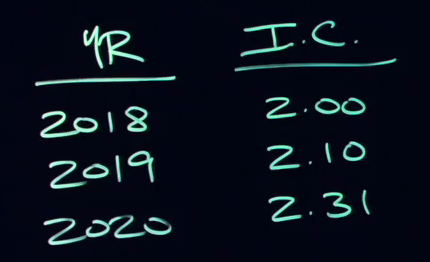
\includegraphics{Chapter2/IceCapCosts.png}
    \caption{Ice Cap Costs Over Three Years}
\end{figure}
\newpage
With an index, we need to select a \emph{base year}.
The base year influences the index number.

Let us assume 2018 is the base year.
\begin{figure}[h!]
    \centering
    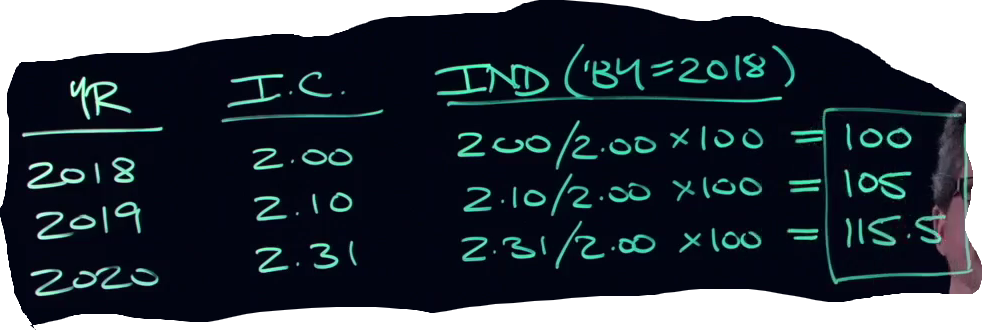
\includegraphics{Chapter2/IceCapIndex.png}
    \caption{Index of Ice Cap Costs Over Three Years, with 2018 as the base year}
\end{figure}
\begin{equation}
    \text{Index} = \frac{\text{Cost in Year X}}{\text{Cost in Base Year}} \times 100
\end{equation}
Composite index is an index made up of multiple items.

Data type sets commonly come in two forms:
\begin{itemize}
    \item \begin{definition}
        \emph{Time series data}, looking at particular data over a period of time.
    \end{definition}
    \item \begin{definition}
        \emph{Cross-sectional data}, looking at a snapshot of data at a particular point in time.
    \end{definition}
\end{itemize}
\newpage
\subsection{}

Economics is math driven.
It is used to describe the real world with models.

\begin{definition}
    \emph{Functions} can be expressed in words, tables, equations or graphs.
\end{definition}
\begin{figure}[h!]
    \centering
    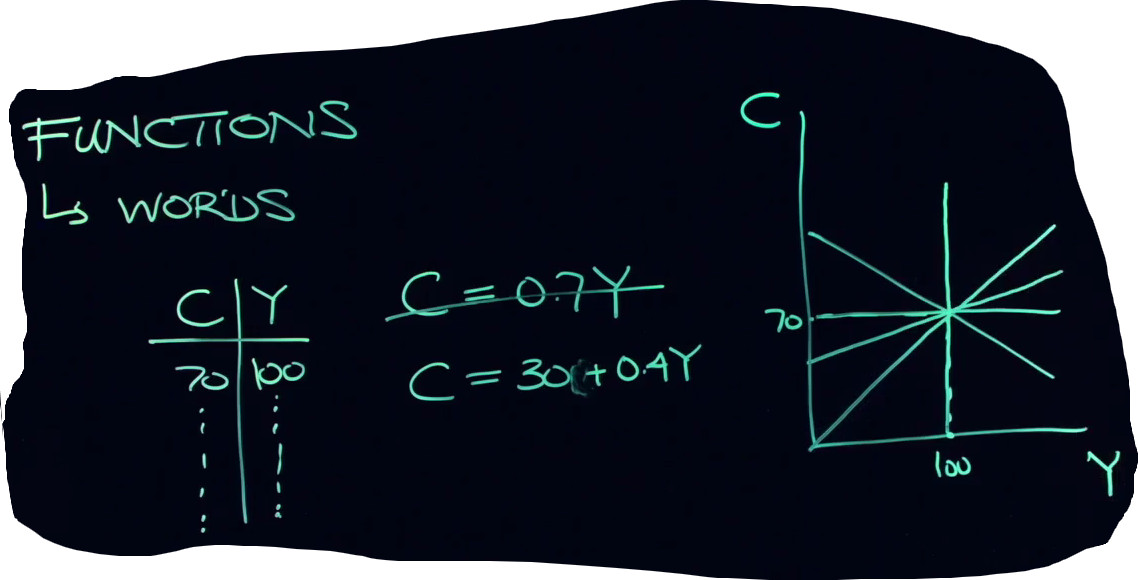
\includegraphics[width=0.75\textwidth]{Chapter2/RepresentationsofFunctions.png}
    \caption{Different Representations of Functions}
\end{figure}
Most of what is done in intro to economics is done with linear functions.
Non-linear functions are interesting because they can be used to find maximum and minimums (optimization).

\section{Chapter 3}
\subsection{}

\begin{definition}
    \emph{Law of demand} says \underline{ceter}is \underline{par}ibus, meaning all things equal. Demand is consumer-driven.
    As the price of something goes up, your willingness to buy it goes down. The reverse is true too,
    as the price of something goes down, your willingness to buy it goes up.\\
    Note: Technically, the law of demand is as the price of something goes up, your willingness to buy it \emph{should not} increase.
\end{definition}
\begin{definition}
    Demand Schedule is a table that shows prices and quantities. Graphing the demand schedule has the 
    quantity as the dependent variable and the price as the independent variable. Even though this is the case,
    Price is on the dependent axis (y-axis) and quantity on the independent axis (x-axis).
\end{definition}
\begin{figure}[H]
    \centering
    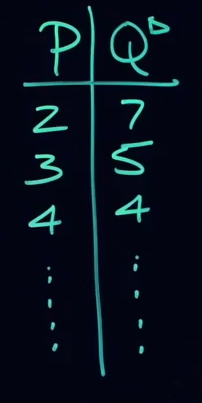
\includegraphics[]{Chapter3/DemandScheduleTable.png}
    \caption{Demand Schedule}
\end{figure}
\begin{definition}
    Demand curve is a graphical representation of the demand schedule. Price is on the y-axis and quantity on the x-axis.
    It is a downward sloping curve, but in the real world it is not always. It is drawn linearly for simplicity, this comes with a problem.
    If the price was free (y=0) it would break the law of demand. Assume the demand curve is for the entire market for the product.
\end{definition}
\begin{figure}[H]
    \centering
    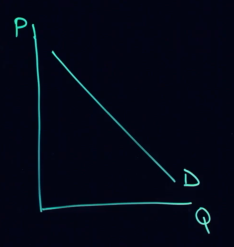
\includegraphics[]{Chapter3/DemandCurve.png}
    \caption{Demand Curve}
\end{figure}
\begin{definition}
    A \emph{shift} in demand is when other factors besides price change.
\end{definition}
\begin{example}
    If your incomes goes up, given the same price of a product, you would want to purchase more of it. (normal good)\\
    Note: There are some goods that you would want to purchase less of if your income goes up (inferior goods). In this event, there would be a left shift.\\
    The demand curve would shift to the right.\\ If a substitute product's price goes up, 
    you would want to purchase more of the original product.
    \begin{figure}[H]
        \centering
        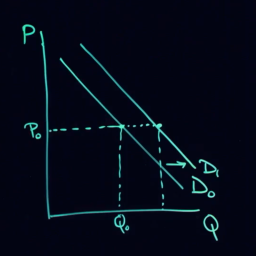
\includegraphics[]{Chapter3/DemandCurveShift.png}
        \caption{Demand Curve Shifts to Right}
    \end{figure}
    If the price of a complementary product goes up, you would want to purchase less of the original product (left shift).\\
    If the price expectation (future price) goes up, you would want to purchase more of the product now.\\
    If the number of consumers increases, demand curve shifts right.\\
    All the above scenarios cause a change in demand.\\
    If the price of the product goes up, the demand curve does not shift. This is only a change in quantity demanded.
\end{example}
\begin{figure}[H]
    \centering
    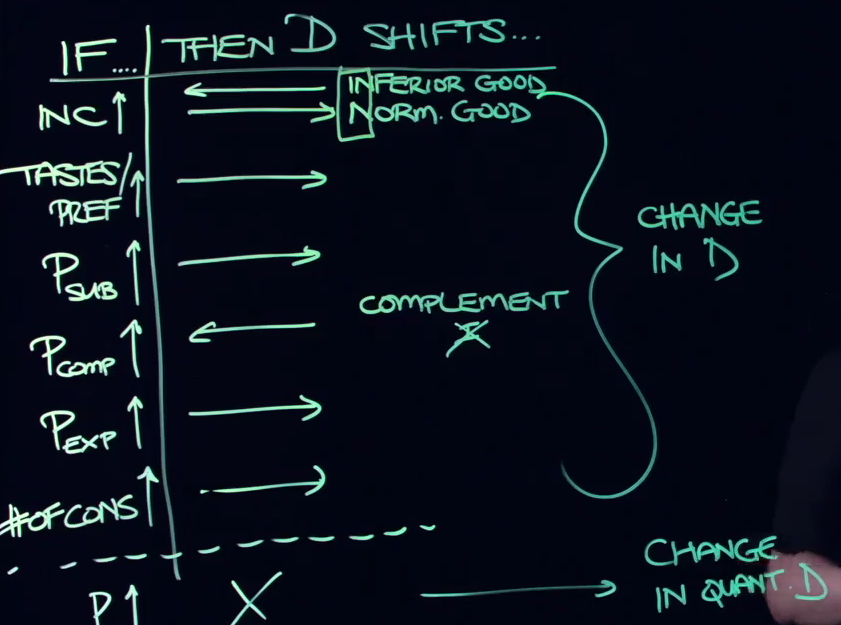
\includegraphics[]{Chapter3/ShiftExamples.png}
    \caption{Demand Shift Examples}
\end{figure}
\newpage
\subsection{}

Remember ceteris paribus
\begin{definition}
    \emph{Law of Supply}, as the price of something goes up, your willingness to produce it goes up.
\end{definition}
\begin{definition}
    \emph{Quantity Supplied}
    \begin{itemize}
        \item The amount of a product that firms \emph{desire} to sell in some time period is called the \emph{quantity supplied}
        of that product.
        \item Quantity supplied is the amount that firms are willing to offer for sale and not necessarily the \emph{quantity actually sold}.
        \item Quantity supplied is a flow as opposed to a stock. 
    \end{itemize}
\end{definition}
\begin{definition}
    \emph{Supply Schedule} is a a table with prices and quantities (subscript s). Your willingness to produce
    a product should not go down as the price goes up. The quantity supplied depends on the price.
\end{definition}
\begin{definition}
    \emph{Supply Curve} is a graphical representation of the supply schedule. Price is on the y-axis and quantity on the x-axis.
    It is an upward sloping curve, it does not need to be linear. The supply curve is for the entire market for the product. 
    There exists a price where the quantity supplied is 0 (reservation price).
\end{definition}
\begin{definition}
    A \emph{shift} in supply is when other factors besides price change.\\
    A \emph{change in supply} is a change in quantity supplied at every price - a shift of the entire curve.\\
    A \emph{change in quantity supplied} refers to a movement from one point on a supply curve to another point - a
    movement along the supply curve.
\end{definition}
\begin{example}
    If price of inputs (resources) are increased, the supply curve shifts left.
\end{example}
\begin{figure}[h!]
    \centering
    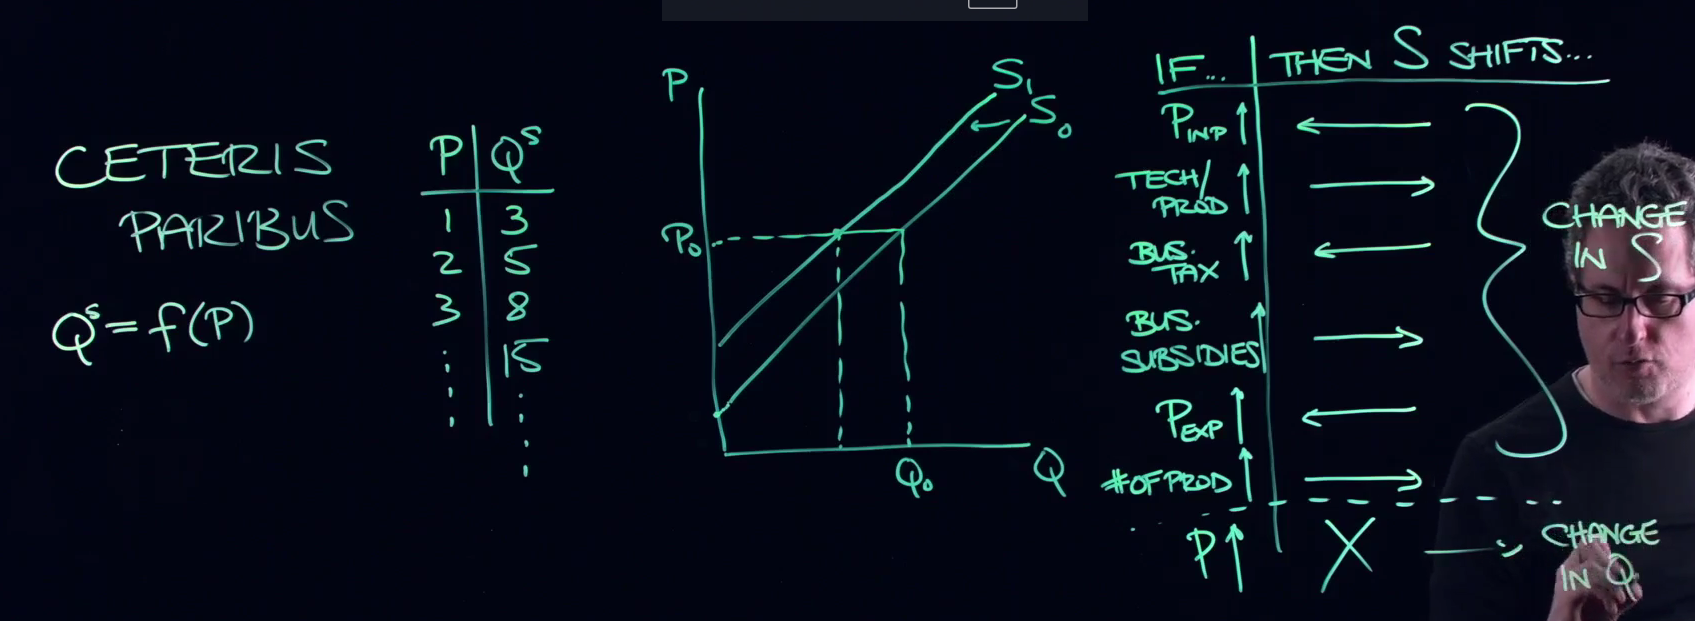
\includegraphics[width=\textwidth, height=\textheight, keepaspectratio]{Chapter3/Supply.png}
    \caption{Supply Information}
\end{figure}
\newpage
\subsection{}

\begin{definition}
    \emph{The equilibrium point} is where the supply and demand curves intersect.
    Price of the product is the variable that brings the market to equilibrium.\\
    $P^*$ and $Q^*$ are the equilibrium price and quantity.\\
\end{definition}
\begin{figure}[h!]
    \centering
    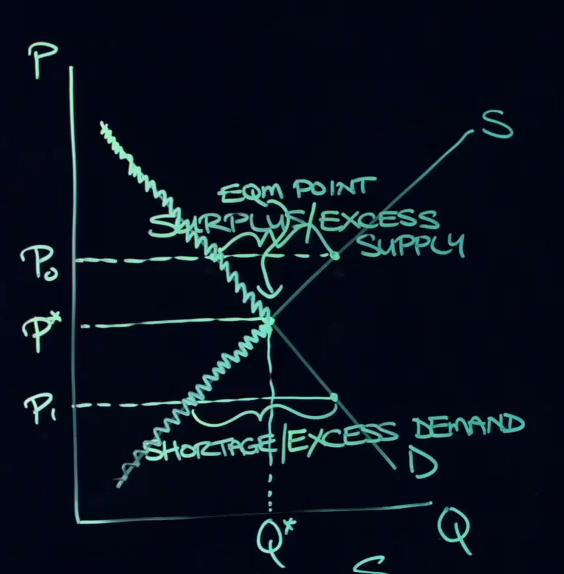
\includegraphics[]{Chapter3/DemandSupplyGraph.png}
    \caption{Demand Supply Graph}
\end{figure}
If prices raise above the equilibrium price, there will be a surplus in supply. If prices fall below the equilibrium price, there will be a shortage.\\
The invisible hand of the market that guides consumers and producers will bring the market back to equilibrium.\\
The short-side (left of $Q^*$) of the market decides what happens.\\
\emph{Laissez faire} is the idea that the government should not interfere with the market.\\
There are 9 different cases of supply and demand shifts.\\
\begin{figure}
    \centering
    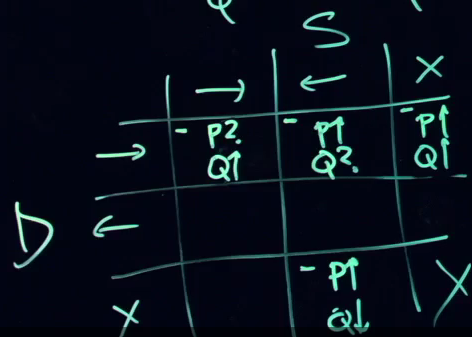
\includegraphics[]{Chapter3/DemandSupplyShifts.png}
    \caption{Demand Supply Scenarios}
\end{figure}
In some scenarios, for example if supply and demand both shift right, the equilibrium price is ambiguous.
The price depends on how much demand or supply shifts right.\\
\begin{figure}[H]
    \centering
    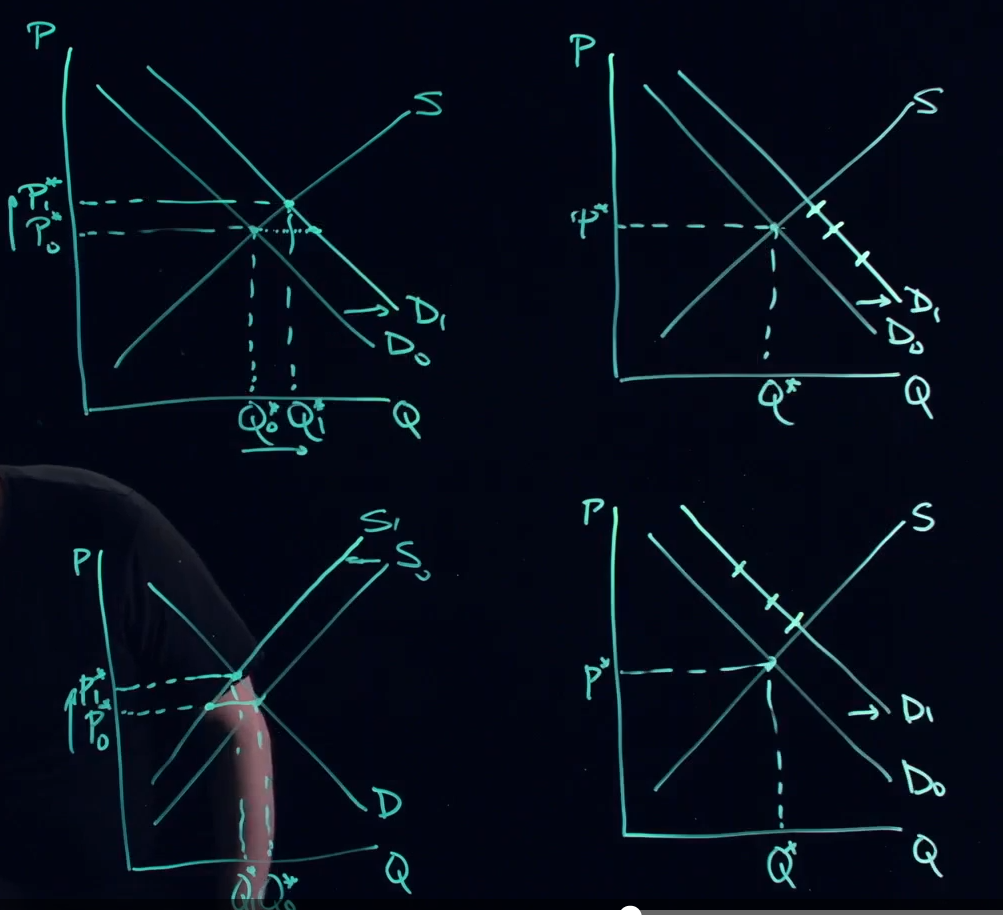
\includegraphics[scale=0.5]{Chapter3/DemandSupplyShiftGraphs.png}
    \caption{Demand Supply Scenarios}
\end{figure}
\newpage
\section{Chapter 4}
\subsection{}

How much does the price and quantity of a product go up or down?
\begin{definition}
    \emph{Elasticity of Demand} is the measure of how much the quantity demanded changes when the price changes.
\end{definition}
Q: If price changes by 1\%, by how much does quantity demanded change (in \%)?\\
A: Price Elasticity of Demand($\eta$).\\
\begin{equation}
    \eta = \frac{\%\Delta Q}{\%\Delta P}=
    \frac{(Q_1 - Q_0)/Q_0}{(P_1 - P_0)/P_0}
    =\frac{Q_1 - Q_0}{P_1 - P_0} \cdot \frac{P_0}{Q_0}=\frac{1}{\text{Slope}}\cdot \frac{P_0}{Q_0}
\end{equation}
When working on price elasticity for demand, the answer is always negative.\\
\[
\eta = 
    \begin{cases}
        \eta = 0\; \text{Perfectly Inelastic}\; \text{e.g. Insulin}\\
        0 < \eta < 1\; \text{Inelastic}\; \text{e.g. Gasoline}\\
        \eta = 1\; \text{Unit Elastic}\; \text{e.g. Lander's mother buying lottery tickets}\\
        1 < \eta < \infty\; \text{Elastic}\; \text{e.g. Non-essential goods}\\
        \eta = \infty\; \text{Perfectly Elastic}\; \text{e.g. PC Cola}
    \end{cases}
\]
Elasticity changes as you move along a given demand curve.\\
There are three basic determinants of elasticity:
\begin{enumerate}
    \item Ceteris Paribus, The more substitutes the product has, the more elastic its demand is.
    \item Ceteris Paribus, the more of your budget this good takes up, the more elastic demand for it is.
    \item Ceteris Paribus, the more time you have to adjust, the more elastic your demand for the product will be.
\end{enumerate}
Elasticity is connected to how much a consumer spends on a product and much revenue a producer makes.
\begin{example}
    If price goes up, then total revenue\dots
    \begin{figure}[H]
        \centering
        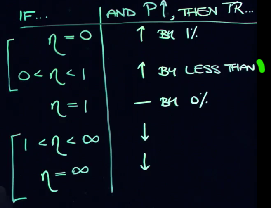
\includegraphics[]{Chapter4/PriceElasticityExamples.png}
        \caption{Price Elasticity Effects on Total Revenue}
    \end{figure}
\end{example}
\subsection{}

\begin{definition}
    \emph{Elasticity of Supply} is the measure of how much the quantity supplied changes when the price changes.
\end{definition}
The determinants are shared with Elasticity of Demand.
\begin{enumerate}
    \item Ceteris Paribus, The more substitutes the product has, the more elastic its demand is.
    \item Ceteris Paribus, the more of your budget this good takes up, the more elastic demand for it is.
    \item Ceteris Paribus, the more time you have to adjust, the more elastic your demand for the product will be.
\end{enumerate}
Consumers and producers can view products differently leading to different elasticities.\\
\subsection{}
What would happen if a tax was introduced into the marketplace?\\
The price the producer receives would be different than the price the consumer pays at equilibrium.\\
\begin{definition}
    \emph{Unit tax} is a fixed amount of tax per unit of the good.\\
    \emph{Ad valorem tax} is a percentage of the price of the good.\\
\end{definition}
\begin{gather}
    t = \text{Unit tax}\\
    P^D = P^S + t\\
    t = P^D - P^S > 0
\end{gather}
Who is paying this tax?\\
\begin{definition}
    {Legal Incidence/Burden} is the person who is legally responsible for paying the tax.\\
    {Economic Incidence/Burden} is the person who actually pays the tax. It is determined by elasticity.\\
\end{definition}
If you are inelastic, you pay more of the tax. If you are elastic, you pay less of the tax.\\
\begin{equation}
    \eta^D < \eta^S \rightarrow \text{Consumers pay more of the tax.}
\end{equation}
\begin{figure}[H]
    \centering
    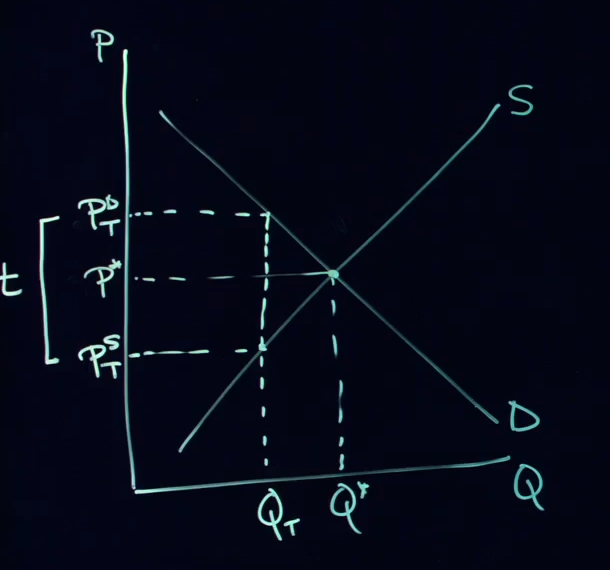
\includegraphics[width=0.5\textwidth]{Chapter4/TaxFiftyFiftyBurden.png}
    \caption{Fifty-Fifty Burden}
\end{figure}
\begin{figure}[H]
    \centering
    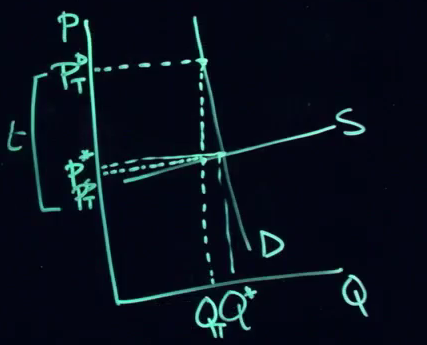
\includegraphics[width=0.5\textwidth]{Chapter4/TaxConsumerBurden.png}
    \caption{Consumer Tax Burden}
\end{figure}
\subsection{}
What if the price that's being changed and the quantity of being affected are different products?
\begin{definition}
    \emph{Cross-price elasticity} is the percentage change in quantity demanded of one good divided by the percentage change in price of another good.
\end{definition}
The sign of the cross-price elasticity matters.
\begin{gather}
    \eta<0 \rightarrow \text{Complements}\\
    \eta=0 \rightarrow \text{Unrelated}\\
    \eta>0 \rightarrow \text{Substitutes}
\end{gather}
What if we are talking about income change instead of price change?
\begin{definition}
    \emph{Income elasticity $(\eta^Y)$} is the percentage change in quantity demanded divided by the percentage change in income.
\end{definition}
\begin{equation}
    \eta=\frac{(Q_1-Q_0)}{(Y_1-Y_0)}\cdot\frac{Y_0}{Q_0}
\end{equation}
\begin{gather}
    \eta>0 \rightarrow \text{Normal Good}\\
    \eta=0 \rightarrow \text{Unrelated to Income}\\
    \eta<0 \rightarrow \text{Inferior Good}
\end{gather}
\section{Chapter 5}
\subsection{}

\begin{definition}
    \emph{Price Controls} usually exist because the government objects 
    to what the market is producing as an equilibrium outcome.
\end{definition}
\begin{definition}
    \emph{Price Floors} are the lowest price you are allowed to pay and charge in the market.
\end{definition}
To bind or make a price floor relevant, it must be above the equilibrium price.
A price floor below or equal to equilibrium is non-binding.\\
The impact of a price floor is a surplus of the good. The issue is that the surplus
cannot go anywhere. The supplier makes the government buy the surplus.\\
The consumers are "losers" because they are not able to buy the good at the equilibrium price.\\
The only "winners" are a small portion of the suppliers.\\
Trying to remove the policy will make the winners vocal.

\subsection{}
\begin{definition}
    \emph{Price Ceiling} is the highest price you are allowed to pay and charge in the market.
\end{definition}
To bind or make a price ceiling relevant, it must be below the equilibrium price.\\
The impact of a price ceiling is that the quantity demanded goes up and the quantity supplied goes down.\\
This creates a shortage of the good.\\
A black market is created because there are consumers willing to pay more than the price ceiling and the price equilibrium.\\
There are a small number of consumers that are "winners" because they are able to buy the good at a lower price.\\
The "losers" are the suppliers because they are not able to sell the good at the equilibrium price.
\subsection{}
\underline{Demand and supply through a new lens}
\par
Demand is a proxy for value. The more you are willing to pay for a good, the more you value it.\\
Supply is a proxy for cost. As long as price covers cost of production, suppliers are willing to produce.\\
Therefore, equilibrium is balancing the value and cost.
\par
The triangle to the left of the equilibrium benefits economic wellbeing. 
It is called total surplus. As a measure of efficiency.
\newline
\begin{figure}[H]
    \centering
    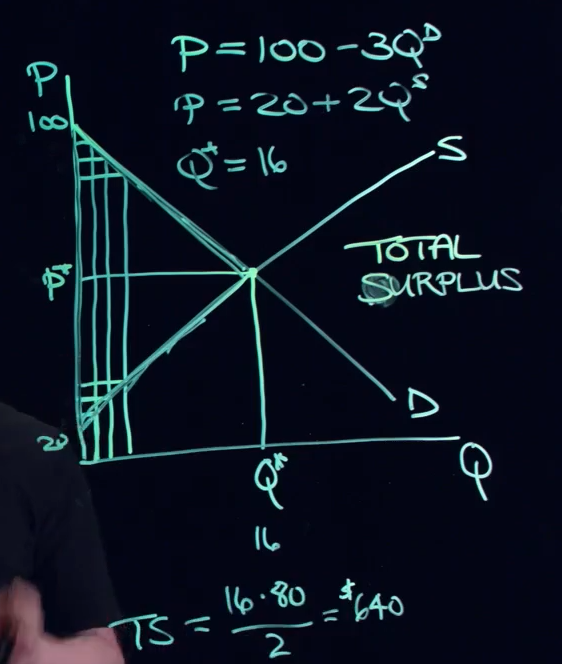
\includegraphics[width=0.5\textwidth]{Chapter5/TotalSurplus.png}
    \caption{Total Surplus}
\end{figure}
Quota is an example of \emph{Quantity Control}. It is a limit on the quantity of a good that can be produced or sold.
\par
The optimal price and quantity control is no price and quantity control.

\section{Chapter 6}
\subsection{}

Where does the demand curve come from?\\
\begin{definition}
    \emph{Utility} loosely is the happiness or satisfaction you get from a good.\\
    It is measured in \emph{utils}. The first good you consume gives you the most utility.
    Each additional good gives you less utility. Each good provides a \emph{Marginal Utility}, 
    which is the additional utility you get from consuming one more good. \emph{Diminishing Marginal Utility} 
    is the idea that the more you consume, the less utility you get from each additional good.
\end{definition}
\begin{figure}[H]
    \centering
    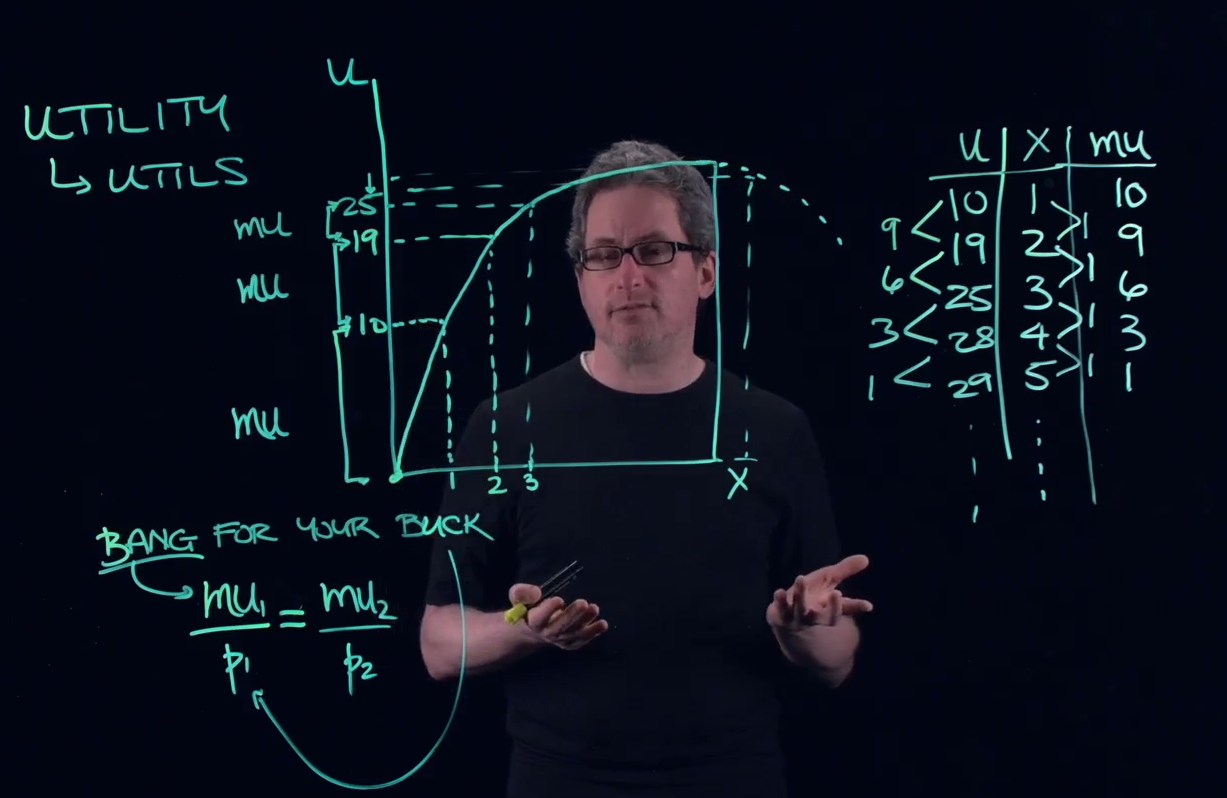
\includegraphics[width=0.5\textwidth]{Chapter6/Utility.png}
    \caption{Utility}
    \label{fig:Utility}
\end{figure}
What if we compare the utility of different goods?\\
We need to factor in the utility and costs.
\begin{equation}
    \begin{gathered}
        \frac{\text{mu}_1}{P_1} > \frac{\text{mu}_2}{P_2}\\
        \frac{\text{mu}_1}{\text{mu}_2} > \frac{P_1}{P_2}\\
        \frac{\text{mu}_1}{\text{mu}_2} = \text{mrs (marginal rate of substitution, how much willing for 1 more good 1)}\\
        \frac{P_1}{P_2} = \text{Relative price ratio (How much you have to give up for 1 more good 1)}\\
        \text{If mrs} > \text{Relative price ratio, you are willing to give up good 2.}\\
        \text{If mrs = Relative price ratio, you are indifferent.}
    \end{gathered}
\end{equation}
After enough transactions the inequality may change.\\
A consumer wants to equalize the equation.
\par
The market demand curve is the sum of all individual demand curves.
\begin{figure}[H]
    \centering
    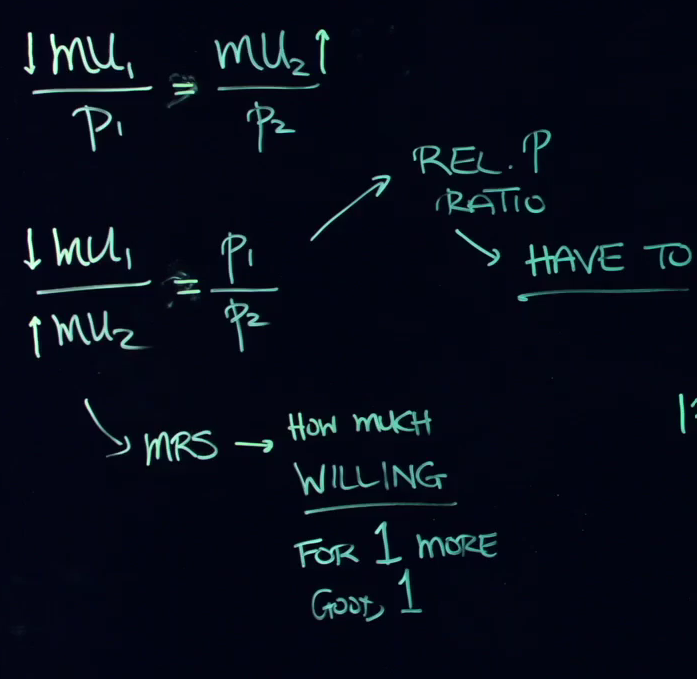
\includegraphics[width=0.5\textwidth]{Chapter6/MarginalUtility.png}
    \caption{Marginal rate of substitution}
    \label{fig:Marginal_rate_of_substitution}
\end{figure}
\par
We assume all consumers are rational and acting in self-interest. Some economists think consumers may be irrational but maybe some consumers are overwhelmed by choice,
or the information is presented in different ways.
\subsection{}
Understanding the logic of what a consumer goes through.
\par
If the price of good 1 goes down, there are two effects.
\begin{enumerate}
    \item Substitution Effect. If purchasing power stays the same, the money will stretch further, either more of good 1 or 2.
    If purchasing power changes with the price change, the consumer would want to purchase more of good 1 and less of good 2.
    \item Income Effect. Based on purchasing power change alone, how does the consumer feel. If the price of good 1 goes down, the consumer is richer.
\end{enumerate}
For a normal good, a price decrease, leads to a higher quantity demanded. But in a more complicated sense,
the consumer substitutes good 1 for good 2 (substitution effect) as well as purchasing more of good 1 due to being richer (income effect).\\
Substitution effect and income effect work in the same direction.
\begin{figure}[H]
    \centering
    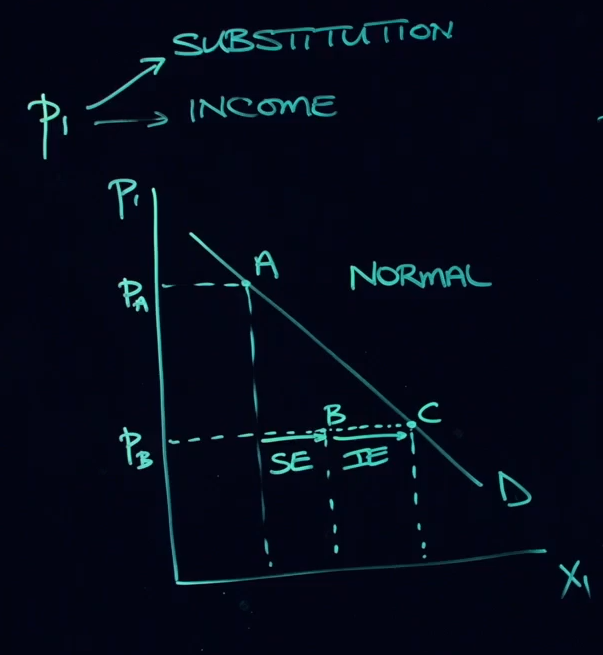
\includegraphics[width=0.5\textwidth]{Chapter6/NormalGood.png}
    \caption{Normal Good}
    \label{fig:Normal_Good}
\end{figure}\par
For an inferior good, a price decrease leads to the substitution effect and income effect working in opposite directions.
The consumer feels richer and doesn't want to buy the inferior good.
\begin{figure}[H]
    \centering
    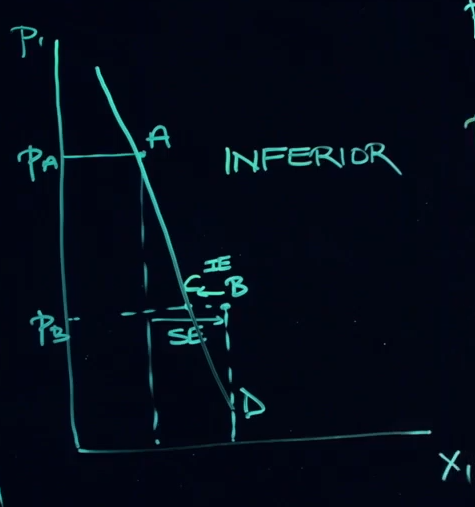
\includegraphics[width=0.5\textwidth]{Chapter6/InferiorGood.png}
    \caption{Inferior Good}
    \label{fig:Inferior_Good}
\end{figure}\par
There is a rare circumstance for an inferior good to be purchased even less after a price decrease.
The income effect outweighs the substitution effect. This is called a Giffen good. Giffen goods must be inferior. The circumstance
requires spending a large amount of income on the good, where the price change sends the consumer after better goods.
\begin{figure}[H]
    \centering
    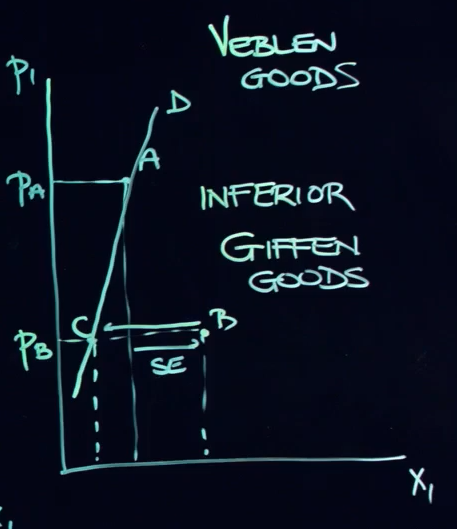
\includegraphics[width=0.5\textwidth]{Chapter6/GiffenGood.png}
    \caption{Giffen Good}
    \label{fig:Giffen_Good}
\end{figure}\par
Another scenario where this could happen is with Veblen goods. These are goods that are purchased for their status or the 
price contains something about the quality of the good.\\
The substitution effect is the change in quantity demanded that results from a change in 
relative prices while 
real income is/are 
constant
. The income effect is the change in quantity demanded that results from a change in 
real income while 
relative prices
is/are 
constant
.
\subsection{}
\begin{definition}
    \emph{Consumer Surplus} is the difference in the maximum the consumer is willing to pay 
    and what is actually paid. Consumer surplus increases for three reasons.
    \begin{enumerate}
        \item the more inelastic the demand curve is.
        \item the lower the price is.
        \item if the demand curve shifts.
    \end{enumerate}
\end{definition}
The maximum willingness to pay is reflected in the demand curve.\\
The consumer surplus is the area under the demand curve and above the price.
\begin{figure}[H]
    \centering
    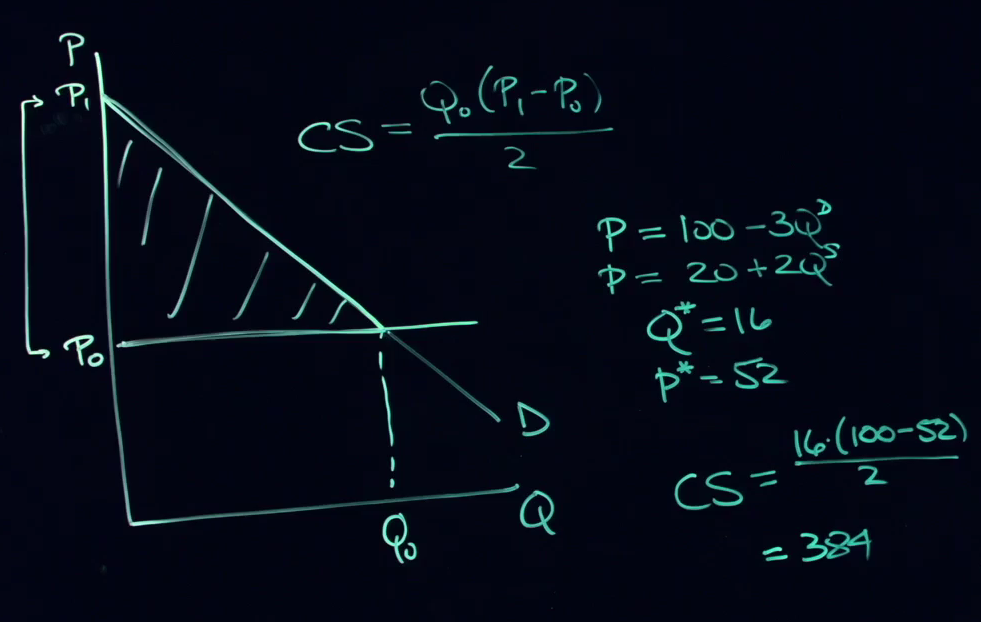
\includegraphics[width=0.5\textwidth]{Chapter6/ConsumerSurplus.png}
    \caption{Consumer Surplus}
    \label{fig:Consumer_Surplus}
\end{figure}
\begin{definition}
    \emph{Paradox of Value}. Think about water being essential for life, but reasonably cheap. Diamonds are not essential, but are expensive.
    The paradox was resolved because water is abundant and diamonds are scarce. We are willing to pay much more for water.
\end{definition}
\begin{figure}[H]
    \centering
    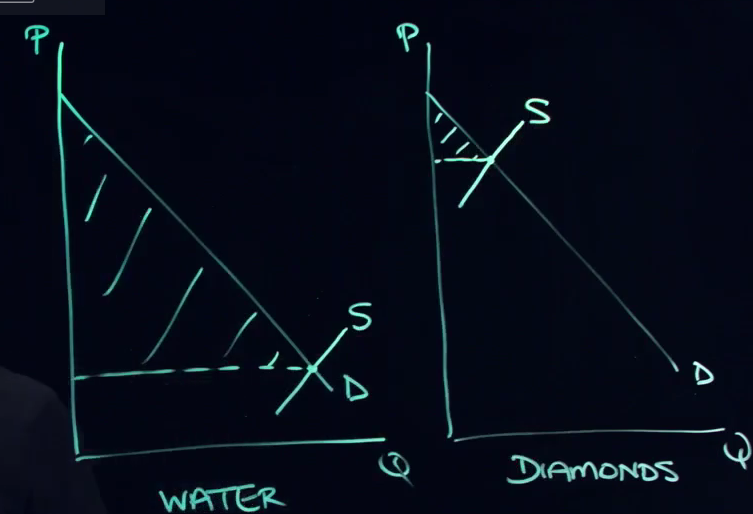
\includegraphics[width=0.5\textwidth]{Chapter6/ParadoxofValue.png}
    \caption{Paradox of Value}
    \label{fig:Paradox_of_Value}
\end{figure}
\subsection*{Appendix A.1}

We need to build up the idea of consumer preferences and taste.
If we compare the quantity of good 1 and good 2, any point or bundle
will provide a certain level of utility. From this bundle, we can compare
utility levels for other bundles. The curve of all points that give the same
level of utility is the idea of an \emph{indifference curve}. There is 
an infinite number of indifference curves for two goods. Extremes are unfavoured.
\begin{enumerate}
    \item The further/highest
    the indifference curve, the higher the utility.
    \item Indifference curves must be downward 
    sloping.
    \item Indifference curves cannot intersect.
    \item Indifference curves must be convex (bow out).
    \item The slope of the indifference curve is -$\frac{MU_1}{MU_2}$ or -MRS.
\end{enumerate}
\begin{figure}[H]
    \centering
    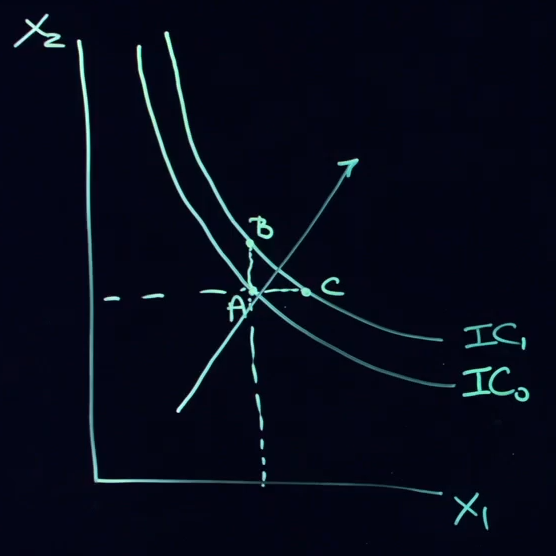
\includegraphics[width=0.5\textwidth]{Chapter6/IndifferenceCurve.png}
    \caption{Indifference Curve}
    \label{fig:Indifference_Curve}
\end{figure}
\subsection*{Appendix A.2}
\begin{equation}
    P_1x_1+p_2x_2 = y
\end{equation}
Where $P_1$ and $P_2$ are the prices of good 1 and good 2 respectively. $x_1$ and $x_2$ are the quantities of good 1 and good 2 respectively. $y$ is the income.\\
If you plot this, the slope is $-\frac{P_1}{P_2}$. This is the budget constraint. Operating within the budget constraint is inefficient, outside is unobtainable. 
\begin{figure}[H]
    \centering
    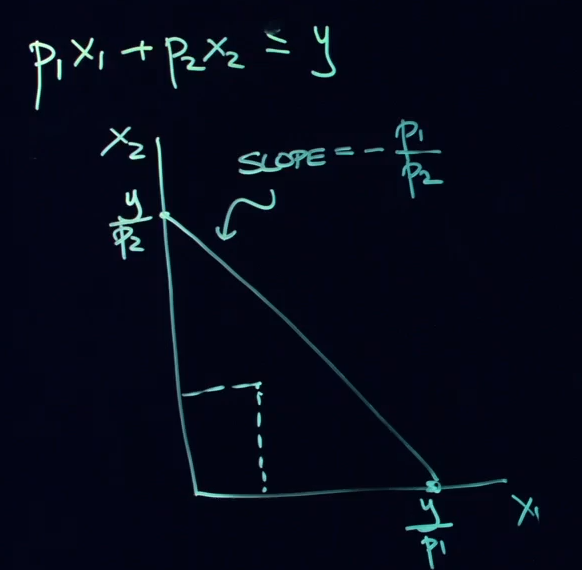
\includegraphics[width=0.5\textwidth]{Chapter6/BudgetConstraint.png}
    \caption{Budget Constraint}
    \label{fig:Budget_Constraint}
\end{figure}
We can combine the constraint with the indifference curve to find the optimal point.\\
There will be some indifference curve with only one point on the budget constraint. This is the optimal point.\\
Where the marginal rate of substitution is equal to the slope of the budget constraint.
\begin{figure}[H]
    \centering
    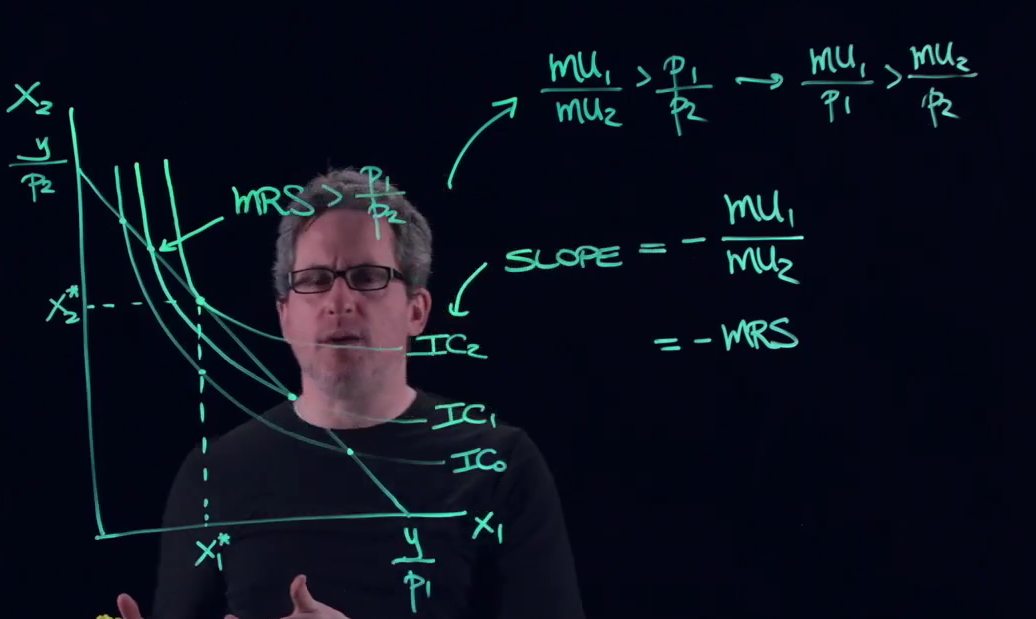
\includegraphics[width=0.5\textwidth]{Chapter6/IndifferenceCurveBudgetConstraint.png}
    \caption{Indifference Curve and Budget Constraint}
    \label{fig:Indifference_Curve_Budget_Constraint}
\end{figure}
\subsection*{Appendix A.3}
If income changes, the budget constraint will shift.\\
Depending on the new optimum, good 1 or 2 may be normal goods or inferior goods.\\
If you connect all the optimal points, you get the \emph{income offer curve}.
\begin{figure}[H]
    \centering
    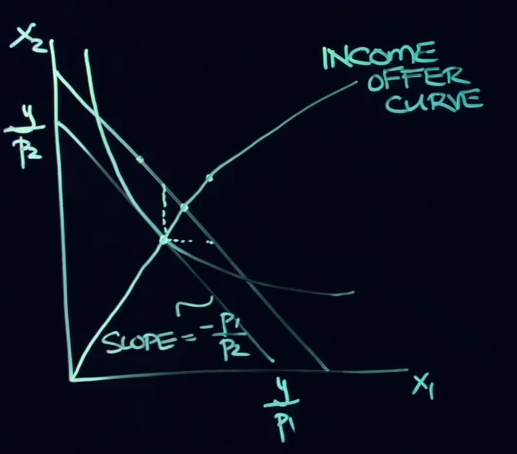
\includegraphics[width=0.5\textwidth]{Chapter6/IncomeChanges.png}
    \caption{Income Offer Curve}
    \label{fig:Income_Offer_Curve}
\end{figure}
If the price of good 1 changes, the budget constraint's slope will change.
If we connect all the optimal points, we get the \emph{price offer curve}.
\begin{figure}[H]
    \centering
    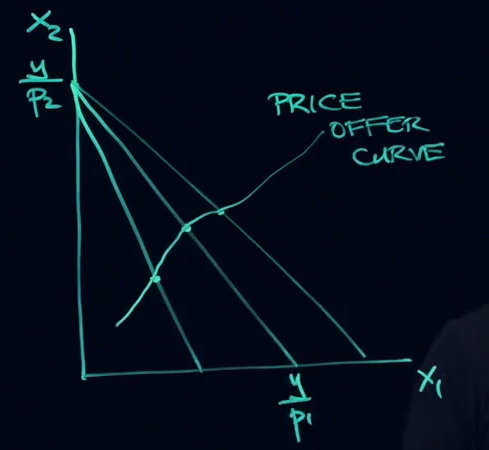
\includegraphics[width=0.5\textwidth]{Chapter6/PriceChanges.png}
    \caption{Price Offer Curve}
    \label{fig:Price_Offer_Curve}
\end{figure}
\subsection*{Appendix A.4}
With the indifference curve and budget constraint,
if price of good 1 decreases, the budget constraints to the right.
Knowing the previous and new optimal points, where do the substitution
and income effect come into play? The substitution effect shows that
the quantity of good 1 and good 2 will change on the tangent of the budget constraint.\\
The income effect is the tangent of the old slope onto the new slope of the budget constraint.
\begin{figure}[H]
    \centering
    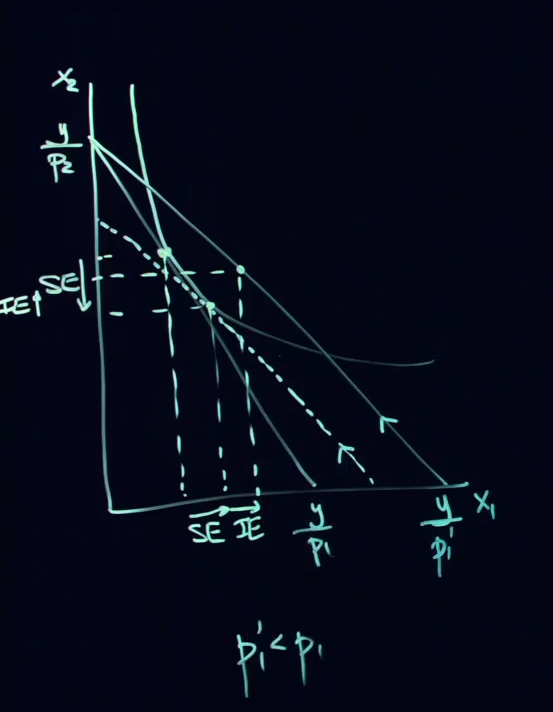
\includegraphics[width=0.5\textwidth]{Chapter6/SubstitutionIncomeEffect.png}
    \caption{Substitution and Income Effect}
    \label{fig:Substitution_Income_Effect}
\end{figure}
\section{Chapter 7}
\subsection{}
Money a firm raises for carrying on its business is called financial capital.\\
The basic types of financial capital used by firms are equity and debt.
The goal of the firm is to maximize profits.\\
We use the greek letter $\pi$ to represent profit.
\begin{equation}
    \pi = \text{Total Revenue}(TR) - \text{Total Explicit and Implicit Costs}(TC)
\end{equation}
\begin{definition}
    Explicit cost, loosely, is something you can get a receipt for.
\end{definition}
\begin{definition}
    Implicit cost are distinctly economics, you can't get a receipt for it but it is a cost for doing business.\\
    For example, if you own a business, the salary you could have earned from your work is an implicit cost.
\end{definition}
Accounting profits are always greater than economic profits.\\
$\pi_A > \pi$.\\
Opportunity cost is contained within implicit cost.
\subsection{}
Inputs that are outputs from some other firm are called intermediate products.
Should firms always maximize profits?\\
Companies that have a higher calling, still need to maximize profits to stay in business.\\
Profits incentivize firms to achieve goals.\\
Total revenue is the price of the product times the quantity sold.
\begin{equation}
    TR = P \times Q
\end{equation}
The amount that a firm produces is equal to amount of resources that the firm has.\\
\begin{equation}
    Q = f(K,L)
\end{equation}
Land is combined with capital.
\par
We can split the production function into two parts, the short run and the long run.\\
The short run is when at least one factors of production are fixed.
Capital is harder to change than labor.
\begin{equation}
    Q = f(\overline{K}, L)
\end{equation}
\par
The long run is when no factors of production are fixed but technology is. The very long run has no fixed factors of production or technology.
\subsection{}
The short run function can take any number of shapes.\\
No workers, no matter the capital, bring no output.\\
As you hire more and more workers, at first the output increases at an increasing rate, then slows down.
\begin{figure}[H]
    \centering
    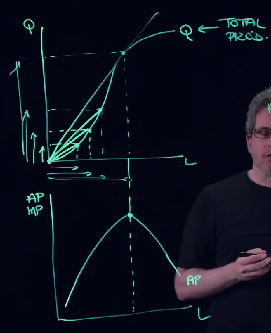
\includegraphics[width=0.5\textwidth]{Chapter7/ShortRun.png}
    \caption{Short Run Production Function}
\end{figure}
\begin{equation}
    \text{Average Production (AP)}= \frac{TP}{L} = \frac{Q}{L}
\end{equation}
The slope of the line from the origin to any point on the short run production curve is the average production.\\
Marginal production is the benefit from hiring one more worker.
\begin{equation}
    \text{Marginal Production (MP)} = \frac{\Delta TP}{\Delta L} = \frac{\Delta Q}{\Delta L}
\end{equation}
One worker means everything they produce is marginal production and the average production.\\
Therefore average production and marginal production are equal at the beginning of the curve.\\
If the average rises, the marginal is above the average.\\
At the maximum point of the average production, the marginal production is equal to the average production.
\begin{figure}[H]
    \centering
    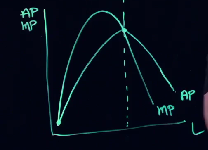
\includegraphics[width=0.5\textwidth]{Chapter7/AverageAndMarginalProduction.png}
    \caption{Short Run Average and Marginal Production}
\end{figure}
We can also see the short run in a table.
\begin{figure}[H]
    \centering
    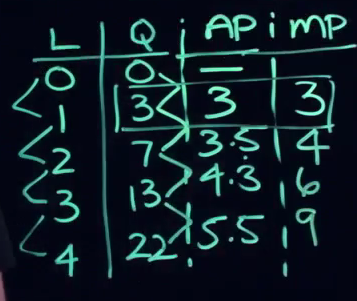
\includegraphics[width=0.5\textwidth]{Chapter7/ShortRunTable.png}
    \caption{Short Run Production Table}
\end{figure}
The AP curve slopes upward when the MP curve is above it.\\
The AP curve slopes downward when the MP curve is below it.\\
The MP curve intersects AP curve at its maximum point.
\subsection{}
Total cost is the sum of total variable cost and total fixed cost.
\begin{equation}
    TC = TVC + TFC
\end{equation}
Or total cost is the sum of the labour and capital costs.\\
Total variable cost is worker wages multiplied by the number of workers.
\begin{figure}[H]
    \centering
    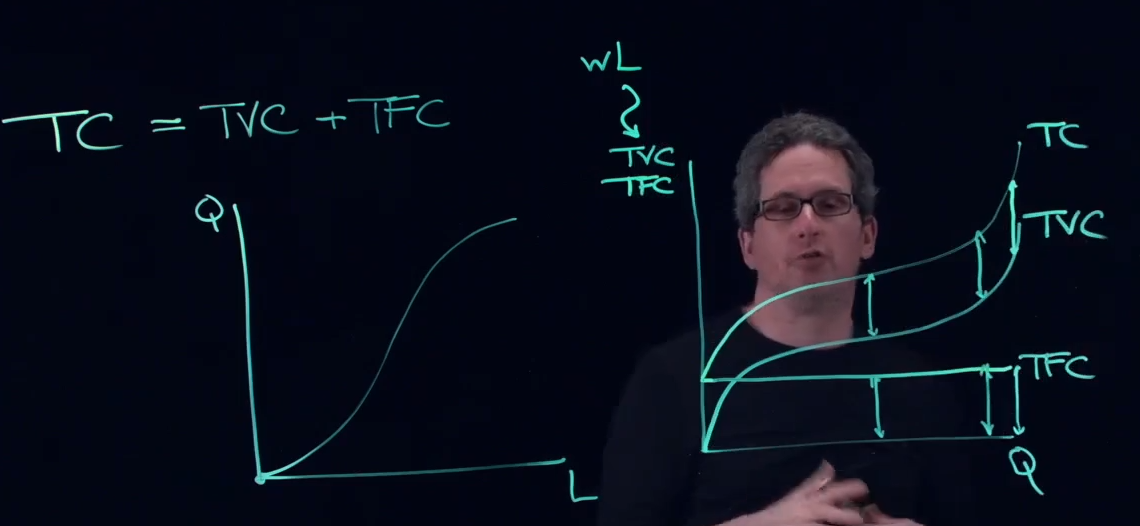
\includegraphics[width=0.5\textwidth]{Chapter7/TotalCost.png}
    \caption{Total Cost}
\end{figure}
\par
The average (total) cost, average variable cost and average fixed cost are found by drawing a linear line from the origin to the total curve.\\
The AC starts at infinity and decreases as the quantity increases.\\
The tangent point of TC must come after the tangent point of TVC.\\
AC and AVC never cross.\\
AFC decreases as quantity increases and can never be zero.
\begin{equation}
    AC = \frac{TC}{Q}
\end{equation}
\begin{equation}
    AVC = \frac{TVC}{Q}
\end{equation}
\begin{equation}
    AFC = \frac{TFC}{Q}
\end{equation}
\begin{equation}
    AC = AVC + AFC
\end{equation}
\par
Marginal cost is the cost of producing one more unit.
\begin{equation}
    MC = \frac{\Delta TC}{\Delta Q} = \frac{\Delta TVC}{\Delta Q}
\end{equation}
\begin{equation}
    MVC = \frac{\Delta TVC}{\Delta Q} = \frac{\Delta TC}{\Delta Q} - \frac{\Delta TFC}{\Delta Q}
\end{equation}
\begin{equation}
    MFC = \frac{\Delta TFC}{\Delta Q} = 0
\end{equation}
\begin{equation}
    MC = MVC
\end{equation}
\begin{figure}[H]
    \centering
    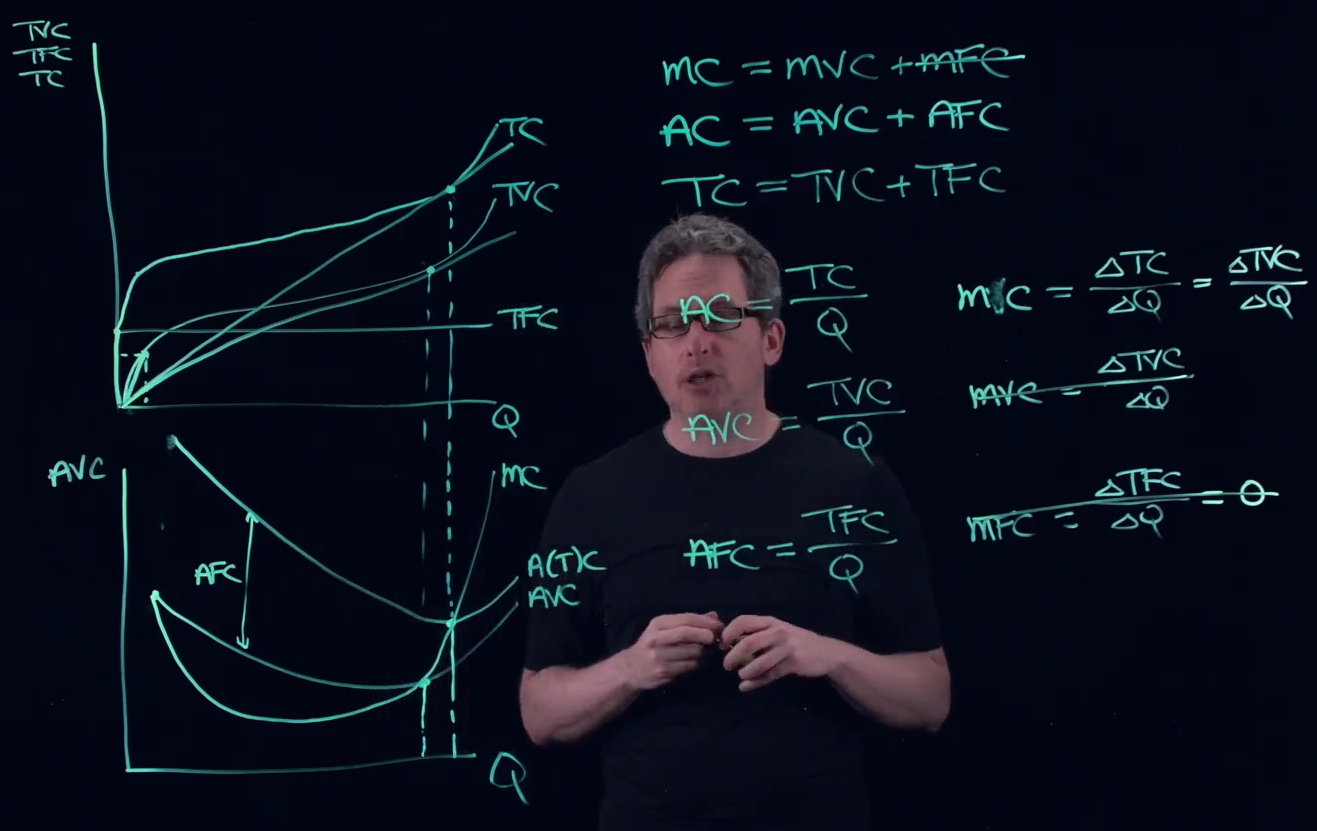
\includegraphics[width=0.5\textwidth]{Chapter7/MarginalCost.png}
    \caption{Average and Marginal Cost}
\end{figure}
\par
\begin{equation}
    MC = \frac{W}{\text{Marginal Product}(MP)}
\end{equation}
\begin{equation}
    MC = \frac{\Delta TC}{\Delta Q}
\end{equation}
\begin{equation}
    \frac{W}{MP} = \frac{W\Delta L}{\Delta Q} = \frac{\Delta TC}{\Delta Q}
\end{equation}
\begin{equation}
    AVC = \frac{W}{AP}
\end{equation}
This can also be represented in a table.
\begin{figure}[H]
    \centering
    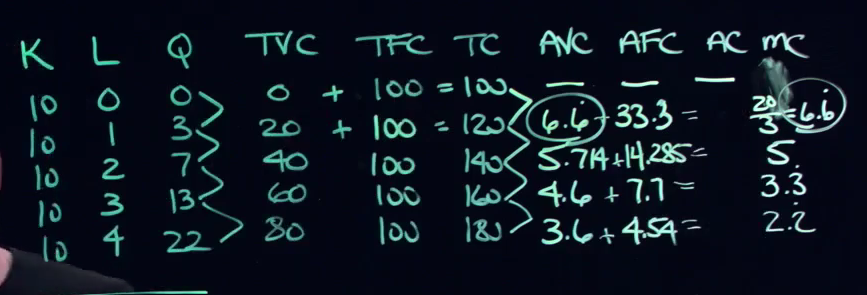
\includegraphics[width=0.5\textwidth]{Chapter7/CostTable.png}
    \caption{Cost Table}
\end{figure}
When AC is at minimum point, profits are maximized.
\section{Chapter 8}
\subsection{}
In the long run, firms can change all their inputs.
Capital and labour are not fixed.\\
They change their inputs in relation to marginal production of capital (MPK) and marginal production of labour (MPL).\\
If MPK $>$ MPL, the firm will increase capital and decrease labour until $\frac{MPK}{P_K} = \frac{MPL}{P_L}$.\\
$\frac{MPK}{P_K} = \frac{MPL}{P_L}$ is called technical efficiency.\\
$\frac{MPK}{MPL} = \frac{P_K}{P_L}$ is called the marginal rate of technical substitution (MRTS).\\
At a given output, minimizing costs maximizes profits.
\par
Long run average cost (LRAC) is connected to the short run average cost (SRAC).\\
Convex hull is the LRAC curve formed from the SRAC curves.\\
Increasing returns to scale (IRS) or economics of scale is when LRAC decreases as output increases (doubling inputs, more than doubles the quantity).\\
Constant returns to scale (CRS) is when LRAC remains constant as output increases (doubling inputs, doubles the quantity).\\
Decreasing returns to scale (DRS) or diseconomies of scale is when LRAC increases as output increases (doubling inputs, less than doubles the quantity).\\
The minimum efficient scale (MES) is the point where CRS begins.\\
Returns to scale come from specialization and division of labour.
\begin{figure}[H]
\centering
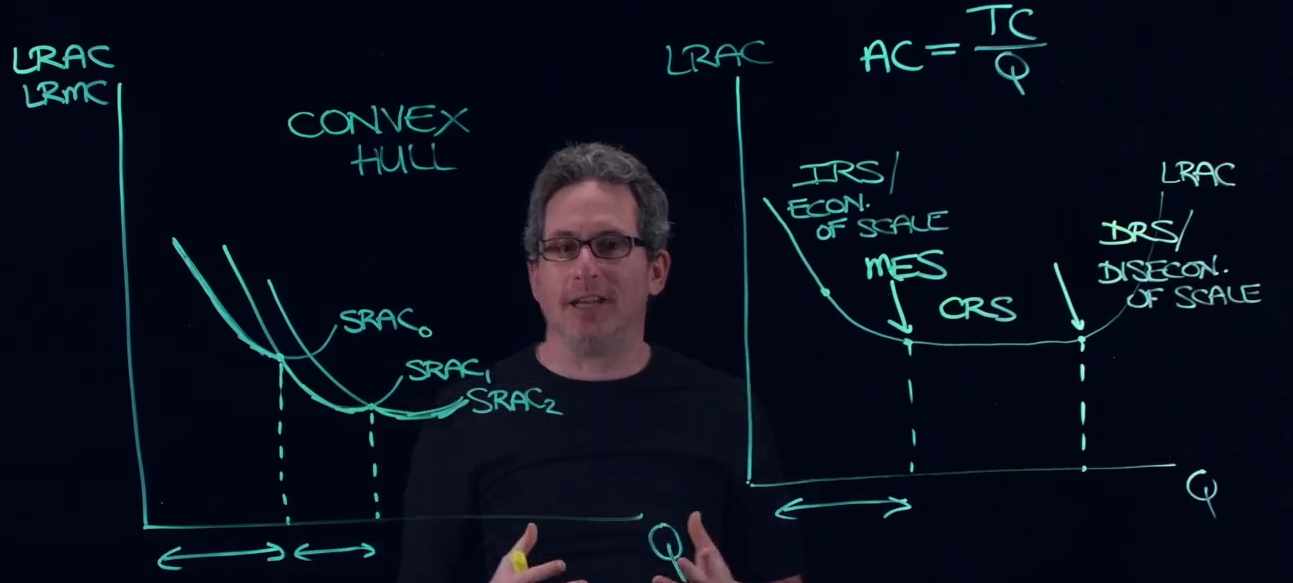
\includegraphics[width=0.5\textwidth]{./Chapter8/LongRunAverageCost.png}
\caption{Long Run Average Cost}
\end{figure}
\subsection*{Chapter 8 Appendix}
Isoquants are curves that show all the combinations of inputs that produce a given output.\\
Isoquants cannot slope up (diminishing marginal products). Isoquants cannot intersect.\\
The slope of an isoquant is $-\frac{MPL}{MPK}$.
\begin{figure}[H]
    \centering
    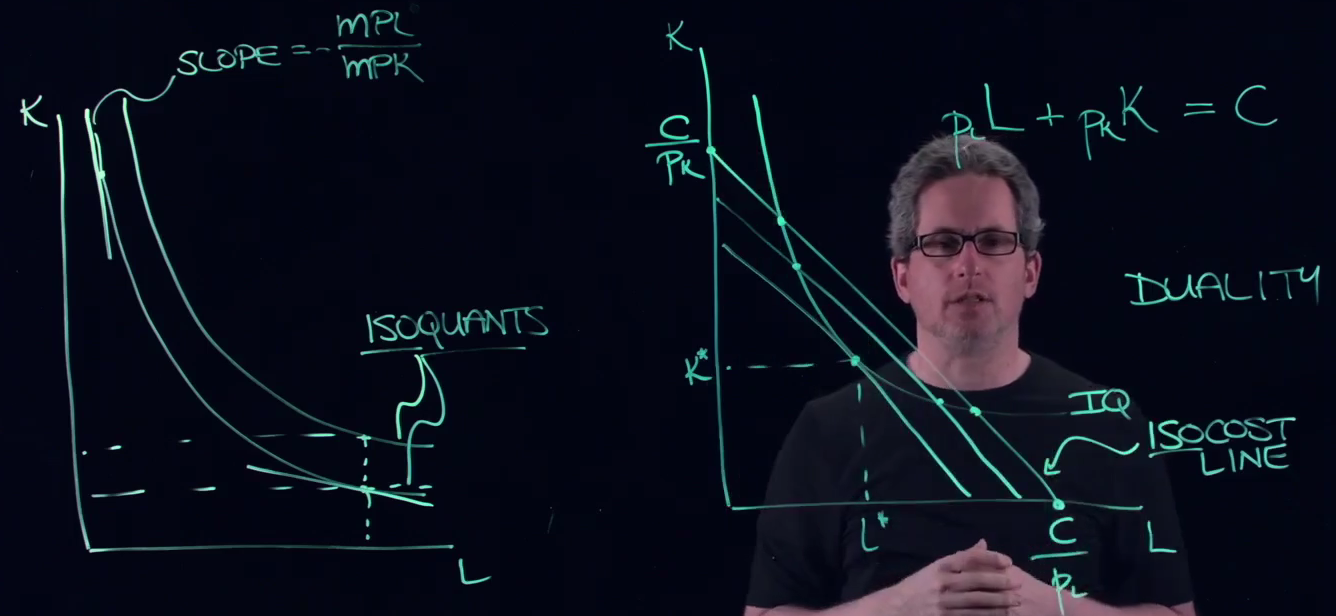
\includegraphics[width=0.5\textwidth]{./Chapter8/Iso.png}
    \caption{Isoquants}
\end{figure}
\section{Chapter 9}
\subsection*{9.1 \& 9.2}
Perfectly competitive markets have 5 assumptions or characteristics.
\begin{enumerate}
    \item All agents within the market are price takers. They cannot influence the price of the good or service.
    \item There are many buyers and sellers in the marketplace.
    \item The product is homogeneous. Everybody in the industry is selling identical products.
    \item There are no barriers to entry or exit. Firms can enter or exit the market freely.
    \item Information is perfect. You may not be fully informed, but what you know, everyone else knows. Equally informed.
\end{enumerate}
Examples of perfectly competitive markets are agriculture and financial markets.
\begin{figure}[H]
    \centering
    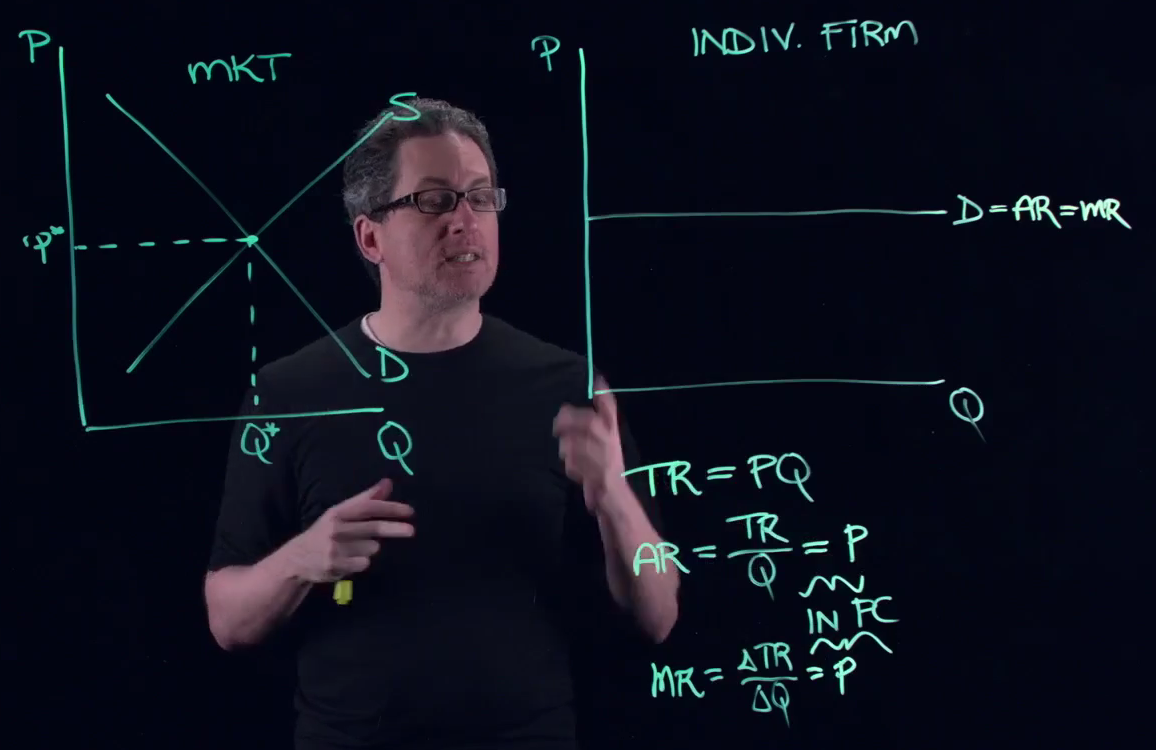
\includegraphics[width=0.5\textwidth]{./Chapter9/PerfectlyCompetitive.png}
    \caption{Perfectly Competitive Market}
\end{figure}
\par
Remember that Total Revenue (TR) is price times quantity.\\
Average Revenue (AR) is TR divided by quantity. In other words Average Revenue is equal to price (in a perfectly competitive market).\\
Marginal Revenue (MR) is the change in Total revenue divided by the change in quantity. In other words, Marginal Revenue is equal to price (in a perfectly competitive market).
\subsection*{9.3}
A firm maximizes revenue for a elastic demand curve by producing where MR = MC, known as the profit maximizing condition.\\
Producing where MR is less than MC is not profit maximizing.\\
Remember AC = $\frac{TC}{Q}$\\
TC = AC$\times$Q\\
AC*, the average cost where MR = MC, must be greater than the minimum.\\
$\pi$ = (P$^*$ - AC$^*$)Q
\begin{figure}[H]
    \centering
    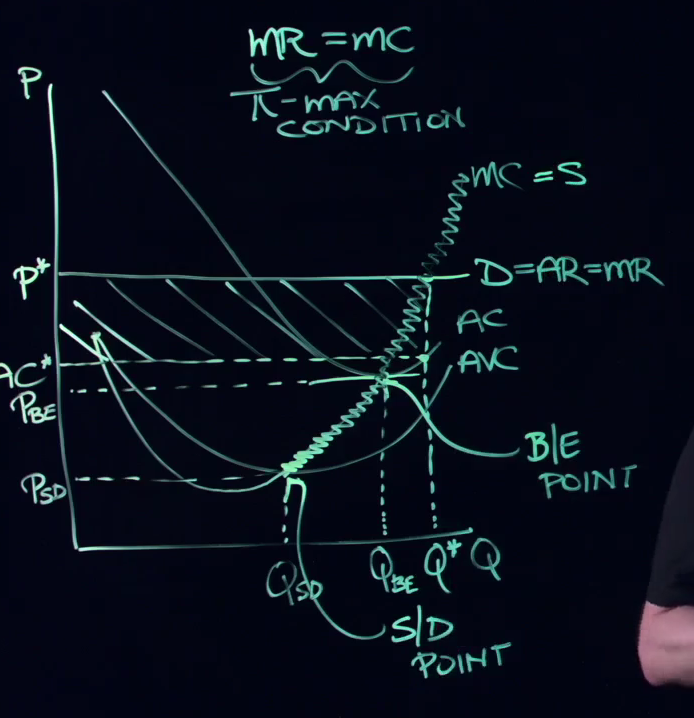
\includegraphics[width=0.5\textwidth]{./Chapter9/ProfitMaximization.png}
    \caption{Profit Maximization}
\end{figure}
The shaded area in the graph is the profits made.\\
If you have multiple intersection points, choose the rightmost.\\
If AC is greater than P, the firm is making a loss.\\
At a loss, the firm cannot pay all of their fixed costs.
\begin{figure}[H]
    \centering
    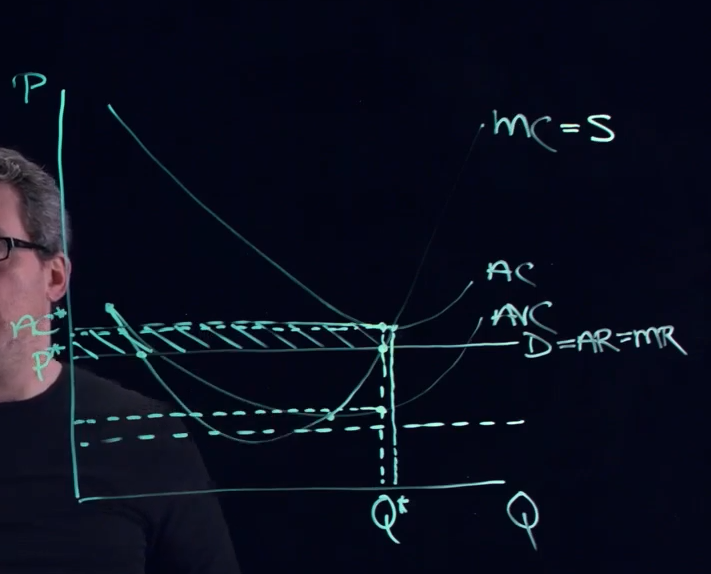
\includegraphics[width=0.5\textwidth]{./Chapter9/ProfitMaximizationLoss.png}
    \caption{Profit Maximization Loss}
\end{figure}
If the quantity at MR=MC intersects with the minimum of the AC curve, the firm breaks even.
This is known as the break even point, break even price and break even quantity.\\
Firms can lose so much money that they can't pay their variable cost.\\
If the quantity at MR=MC intersects with the minimum of the minimum of the AVC curve, this is the shut down point, shut down price and shut down quantity.\\
Marginal Cost curve is in fact the supply curve, as long as it is above the shut down point, otherwise the quantity supplied is 0. The reservation price is the shut down price.
\subsection*{9.4}
In the long run, if one firm is profiting, all firms are profiting. Based off the assumptions made, this means new firms will join the market.\\
This will shift the supply curve to the right, lowering the equilibrium price. Profits will lower.\\
Firms will keep entering the industry until the profit is gone.
\par
If one firm is losing, all firms are losing. Based off the assumptions made, this means firms will leave the market.\\
This will shift the supply curve to the left, raising the equilibrium price. Losses will lower.\\
Firms will keep leaving the industry until the loss is gone.\\
In the long run, firms cannot make a profit or a loss, in the short run, you can.\\
$\pi=0$, $\pi_{\text{Accounting}}>0$. This is called the normal profit.\\
In the long run, the LRAC curve is driven down where the MC curve intersects with the minimum LRAC curve.
\begin{figure}[H]
    \centering
    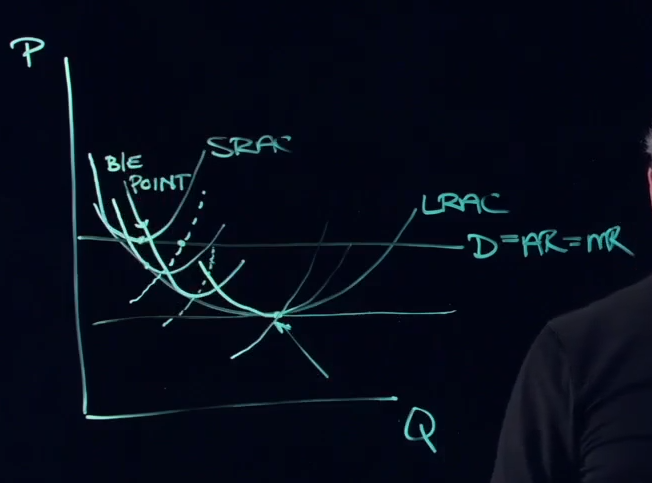
\includegraphics[width=0.5\textwidth]{./Chapter9/LongRunProfitMaximization.png}
    \caption{Long Run}
\end{figure}
Those who can quickly implement technology advances are those who profit.\\
If the taste or preferences of consumers move away from your product. Those who 
leave quickly or adapt to the price, will be able to hang on without losing money.\\
Those who are slow will lose more quickly.
\section{Chapter 10}
\subsection{}
A monopoly market is the opposite of a perfectly competitive market.\\
A monopoly has 5 assumptions or characteristics.
\begin{enumerate}
    \item The firm is a price maker.
    \item Many buyers and one seller.
    \item Heterogeneous product. The product is unique.
    \item Barriers to entry and exit. Firms cannot enter or exit the market freely.
    (i.e. entry: ownership of a resource, high startup costs, economies of scale, predatory pricing, the government itself,
    exit: government doesn't allow monopolist to leave)
    \item (Im)perfect information.
\end{enumerate}
Examples of monopolies are Canada Post, train and metro systems.\\
Price discriminating monopolies and single price monopolies are the two types of monopolies.\\
Price discriminating examples include student discounts on the metro.\\
For a single price monopoly, the market graph is the same as the individual firm.
The demand curve is equal to the average revenue curve.\\
The marginal revenue curve is twice as steep as the demand curve, when the demand curve is linear.\\
The market will produce where marginal cost equals marginal revenue.\\
The average cost is where the quantity produced intersects the average cost curve.\\
The profit is the area between the average cost curve and the demand curve.\\
The break even point in a monopoly is NOT the minimum of the average cost curve.\\
Monopolies can profit, loss or break even but cannot shut down.\\
In the long run, it is possible for a monopoly to make a profit or a loss.\\
The price charged by a monopoly is higher than the price charged if it were a perfectly competitive market.
\begin{figure}[H]
    \centering
    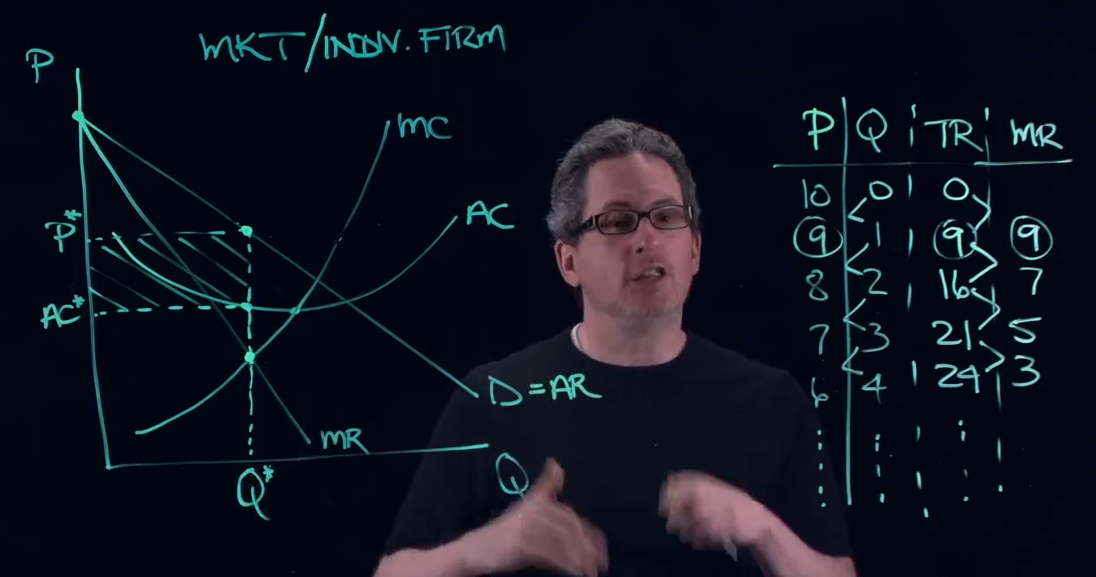
\includegraphics[width=0.5\textwidth]{Chapter10/MonopolyGraph.png}
    \caption{Monopoly Market}
    \label{fig:monopoly}
\end{figure}
\subsection{}
A cartel is when multiple companies come together to form a monopoly.\\
Cartels are unstable and don't last long.\\
Each company in the cartel has a temptation to produce more than the agreed upon quantity, to sneak a profit.\\
\par
The barriers to entry today may be temporary, with technological advances they may fall.
\subsection{}
The monopolist has perfect information in a price discriminating monopoly.\\
In order for price discrimination to exist, 4 scenarios must exist:
\begin{enumerate}
    \item The demand curve must be downward sloping.
    \item Monopolists need to be able to segment their markets. (i.e. student discounts)
    \item Consumer response (elasticity) must be different.
    \item Monopolists need to prevent resale.
\end{enumerate}
Marginal Revenue will be different in a price discriminating monopoly.\\
The demand curve is equal to marginal revenue.\\
The price discriminating monopoly produces more than a single price monopoly.\\
The price discriminating monopoly produces the same amount as a perfectly competitive market.\\
The price discriminating monopoly price charged is a range between the demand curve and the marginal cost curve.\\
Price discriminating monopoly will always be more profitable than a single price monopoly.\\
Total revenue in a price discriminating monopoly is calculated by adding the total revenue of each segment. It is not simply P $\times$ Q\\
MR = D.
\begin{figure}[H]
    \centering
    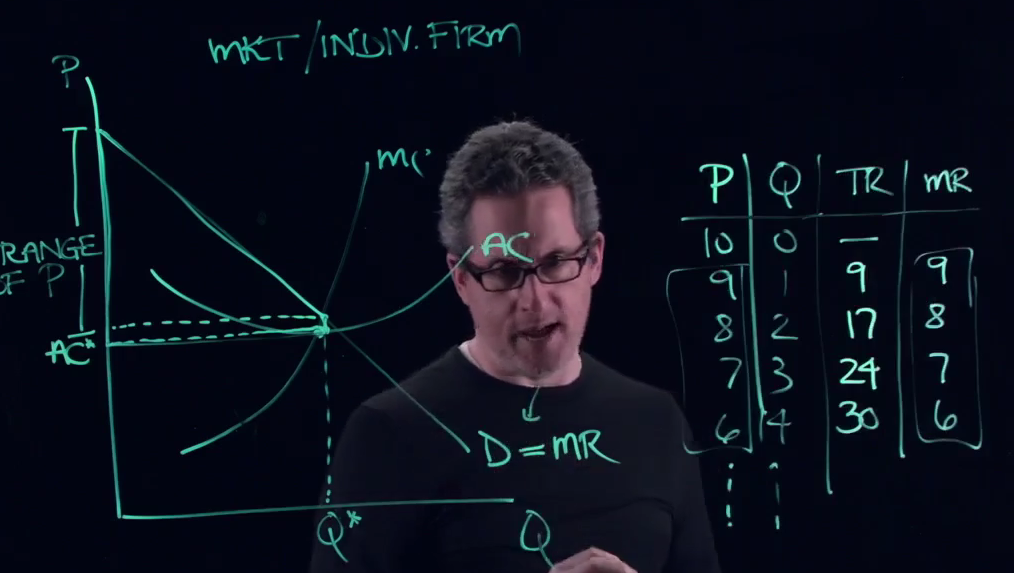
\includegraphics[width=0.5\textwidth]{Chapter10/PriceDiscrimination.png}
    \caption{Price Discriminating Monopoly}
    \label{fig:pricediscriminating}
\end{figure}
The more inelastic the demand curve, the higher the price charged and higher the profit.\\
\section{Chapter 11}
\subsection{}
In imperfect competition, you either have many small firms (monopolistic competition) or few large firms (Oligopoly).
\par
A concentration ratio is the percent of sales go to the top firms. The more sales that are taken from higher firms means it is more monopolistic and less perfectly competitive.
\par
Imperfect competitions have differentiated products (e.g. fast food burgers). The more differentiated the product is the more monopolistic the market.
\par
Imperfect competition has some degree of price-making power. Exerting too much influence leads to your competitors punishing you. Firms compete in ways other than price. They compete through
advertisements, quality and the basis of creating barriers (exclusivity).
\subsection{}
There comes 5 assumptions with monopolistic competition,
it is a hybrid of monopoly and perfect competition.
\begin{enumerate}
    \item Price makers.
    \item Many buyers and many sellers (still not as many as perfect competition).
    \item The product is heterogeneous (differentiated).
    \item No barriers to entry or exit.
    \item Imperfect information.
\end{enumerate}
Examples of monopolistic competition are fast food restaurants, clothing stores and gas stations.
Advertising exists because of the differentiation of products.
\par
Demand is downward sloping but more elastic than a monopoly.\\
The demand curve is equal to average revenue.\\
The marginal revenue curve is twice as steep as the demand curve.\\
The shut-down point exists but is not important to know it's location.\\
Marginal cost intersects the minimum of the average cost curve.
\begin{figure}[H]
    \centering
    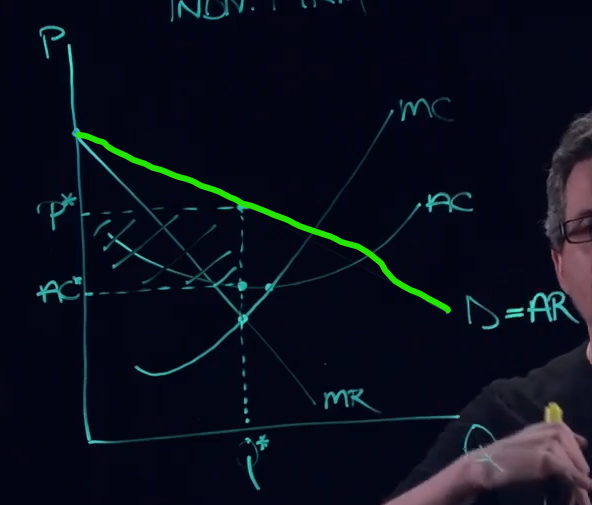
\includegraphics[width=0.5\textwidth]{Chapter11/MonopolisticCompetition.png}
    \caption{Monopolistic Competition}
    \label{fig:monopolisticcompetition}
\end{figure}
If a firm is making a profit in monopolistic competition, other firms will enter the market.\\
If a firm is making a loss in monopolistic competition, the firm will exit the market.\\
All firms in the long run will break even.
\par
A monopolistic competition has a trade off with perfect competition.
In exchange for operating below optimal efficiency, the consumer has to pay a premium for having choice between
differentiated products. If firms increased production, they would give up the differentiation.\\
The concept of firms in a monopolistic competition operating below optimal efficiency is called excess capacity.
\subsection{}
Oligopolies have 5 assumptions:
\begin{enumerate}
    \item Price makers.
    \item Many buyers and few sellers.
    \item Heterogeneous product (differentiated).
    \item Barriers to entry and exit.
    \item Imperfect information.
\end{enumerate}
Examples of oligopolies are Canadian banking industry.\\
Two firms in an oligopoly is called a duopoly.
\par
Strategic interdependence is when firms are aware of the actions of other firms and take that into account when making decisions.\\
Game theory is used to analyze the strategic interactions between firms.\\
A payoff matrix is a table that shows the payoffs for every possible action by each player.\\
We will look at an example with two firms and two strategies.\\
Firm B has the ability to announce to cooperate with firm A or compete.\\
Firm A has the ability to cooperate with firm B or compete.\\
A dominant strategy is a strategy that is best for a player in a game regardless of the strategies chosen by the other players.
Nash equilibrium is that the players do not want to change their strategy after it has been chosen.
\begin{figure}[H]
    \centering
    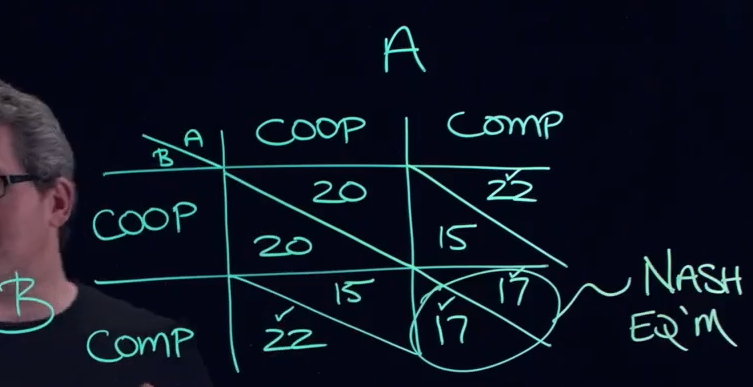
\includegraphics[width=0.5\textwidth]{Chapter11/GameTheory.png}
    \caption{Game Theory}
    \label{fig:gametheory}
\end{figure}
In this example, the Nash equilibrium is for both firms to compete (compete-compete).
\subsection{}
What if the player's in a game try to collude?\\
In an overt (out in the open) collusion, the government will get involved, because competition is good for the consumer.\\
The alternative is tacit (quiet or implied) collusion.
\par
Collusion works best if there is monitoring and enforcement.
\par
In oligopolies, the firms are making profits, prices are above costs, meaning they would collude to prevent other firms from entering the market.
\par
Barriers can be seen as branding (veblen goods).\\
Advertising is an extension of branding.\\
Advertising is getting a consumer to buy something they would otherwise not buy.\\
This is damaging to the consumer's utility and economic efficiency.\\
Most advertising is deceptive.
\par
Predatory pricing is when a firm threatens to lower prices to drive out competitors.
\section*{16 Chapter 16}
\subsection*{16.1 \& 16.2}
We will look at the government, the third party, in this chapter.
\par
In order for a government to be able to create a functioning economy, 
they need to have a monopoly on violence. Only the government can have an army,
police force, legal system, etc...
\par
Society decides the appropriate level of monopoly power for the government.
\par
The government needs to create an informal defense on how the society operates.
By creating a monopoly on violence, any change in supply and demand are going to 
find their way towards a new equilibrium.
\par
The government's monopoly allows for innovation and development in the economy.
Innovation leads to profit because the government gives you patents.
\par
The government needs to balance its grip on the economy.
The grip can change over time.
\subsection*{16.3}
There are cases where the governments needs to go beyond its monopoly on violence 
and its encouragement of the free market and actually get involved in the market.
\par
For example when there is market power. Pricing above marginal costs is inefficient.\\
This is why patents, trademarks, and copyrights expire.
\par
Another example is when there is an externality present. Externalities can be on the demand or supply side and also be positive or negative.\\
This can be graphed to show marginal benefits and marginal costs.\\
The government introduces taxes and subsidies to deal with externalities.\\
Taxes and subsidies don't only have to come from the government. They can come from the private sector as well.
\begin{figure}[H]
    \centering
    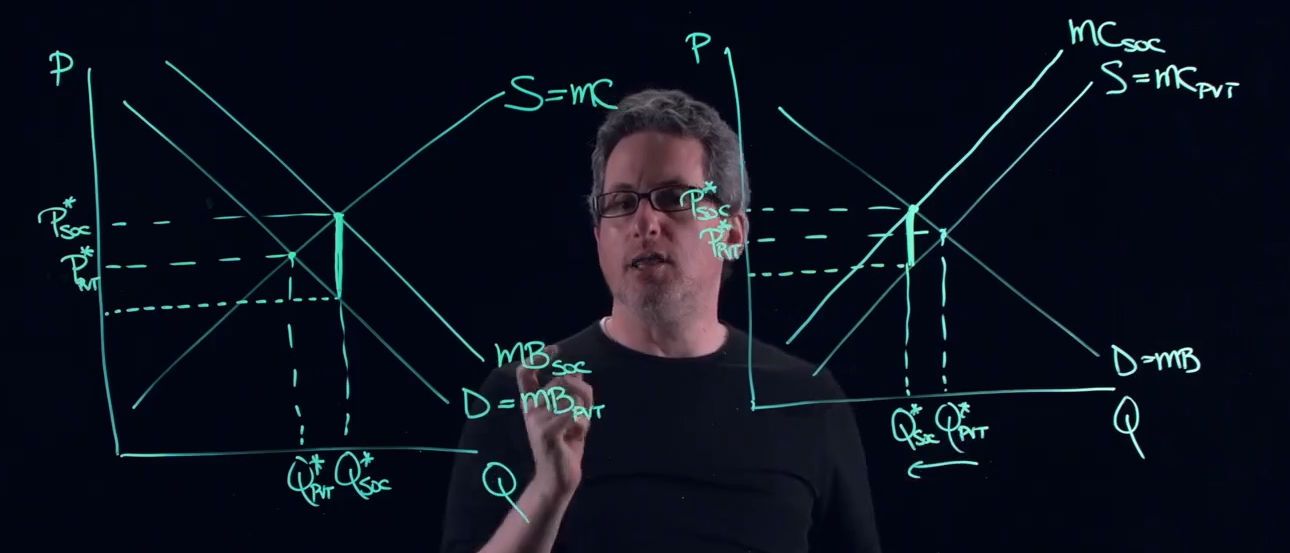
\includegraphics[width=0.5\textwidth]{Chapter16/externalities.png}
    \caption{Externalities}
    \label{fig:externalities}
\end{figure}
Every good or service can be described as rival in consumption or non-rival in consumption.\\
They are also excludable or non-excludable.\\
Excludable good means that you can prevent someone from using it.\\
Rival in consumption means that if you use it, I can't use it.\\
Most of what we look at it is excludable and rival in consumption.
\begin{figure}[H]
    \centering
    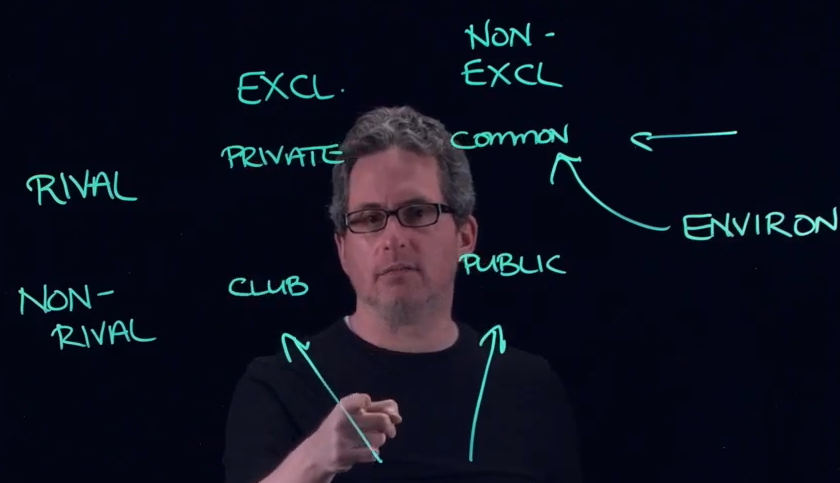
\includegraphics[width=0.5\textwidth]{Chapter16/Goods.png}
    \caption{Goods}
    \label{fig:goods}
\end{figure}
Club and public goods may require government intervention.\\
The government may provide subsidies for club goods.
\par
Public goods are characterized by free riding.\\
The government sums the individual demand curves vertically to get the market demand curve.\\
The issue is that the government does not know the individual demand curve sso they tax everyone.
\begin{figure}[H]
    \centering
    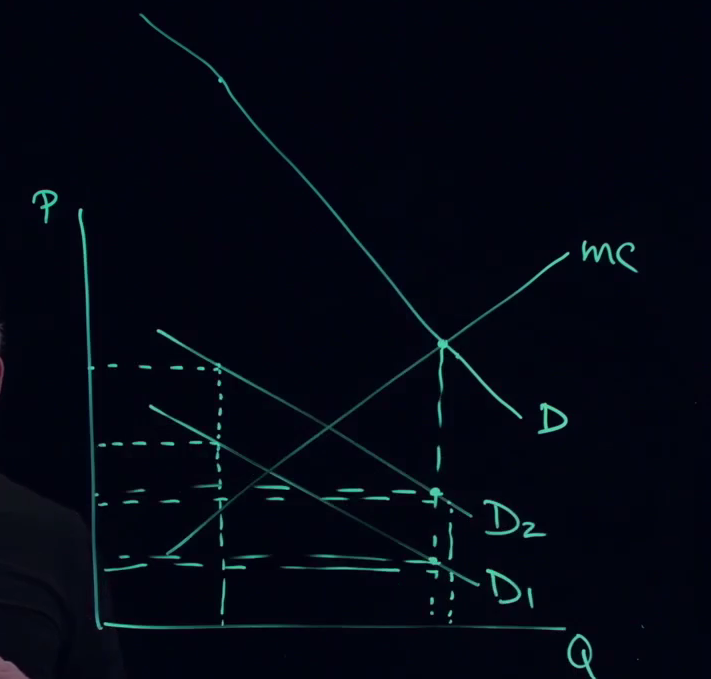
\includegraphics[width=0.5\textwidth]{Chapter16/PublicGoods.png}
    \caption{Public Goods}
    \label{fig:publicgoods}
\end{figure}
Information is excludable and non-rivalrous.\\
Knowledge is non-excludable and non-rivalrous.
\par
Asymmetric information is when one party knows more than the other party.\\
Two things come from this:
\begin{itemize}
    \item Adverse selection: occurs before a transaction takes place. 
    \item Moral hazard: occurs after a transaction takes place.
\end{itemize}
We deal with this by trying to symmetrize the information.
\subsection*{16.4}
In every case except for public goods, there is a market mechanism that could come up with an efficient
way to allocate limited resources from those who value it the goods the least to those who value it the most.
\par
One of the roles of the government is to make sure that the distribution of goods is equitable.
Society has to decide the amount of efficiency to sacrifice for equitable distributions.
\par
The government might exist merely because society wants it to exist. They want the government deal with the distribution of goods.
Society might not trust the private market to do a job, so they have the government do it.
\par
Another reason why the government may need to play a role in the market, consider education. All children must be in school till a certain age.
They are protecting the children from their parents who might not want to send them to school.
\par 
We may need to even be protected from ourselves.
\par
There are some goods where the market mechanism shouldn't exist. For example, the market for grades.
\section*{19 Chapter 19}
\subsection*{19.1}
International trade has no ambiguity, it is good and has the ability to make everyone better off.\\
Free trade means voluntary exchange between two countries.\\
The gain from free trade is always greater than the loss.\\
Closing borders gives market power to the producers and they can charge higher prices.\\
The difference between the price of an "evil" product and its counterpart shows how much society values the cause of the counterpart.
\par
David Ricardo created a model that shows how two countries can benefit from trade.\\
Imagine two countries, and two goods.\\
Trade is not based on absolute advantage, but comparative advantage.\\
A country that doesn't trade is called autarky.
\begin{figure}[H]
    \centering
    \includegraphics[width=0.5\textwidth]{Chapter19/ComparativeAdvantage.png}
    \caption{Comparative Advantage}
    \label{fig:comparativeadvantage}
\end{figure}
In this example, Mexico should export tacos, and Canada should export beer.\\
Open to trade means open to immigration and emigration too.
\par
Outside of autarky, the price of a good falls between the two countries.
\begin{figure}[H]
    \centering
    \includegraphics[width=0.5\textwidth]{Chapter19/GlobalPrice.png}
    \caption{Global Price}
    \label{fig:globalprice}
\end{figure}
\par
We can also look at the production possibility frontier with the budget constraint and indifference curve for the entire country in autarky.\\
The excess or shortage of a leads to export/imports.\\
This won't work in the real world because the declining industry will protest.
\begin{figure}
    \centering
    \includegraphics[width=0.5\textwidth]{Chapter19/PPF.png}
    \caption{Production Possibility Frontier}
    \label{fig:ppf}
\end{figure}
\par
Some countries have a comparative advantage due to natural resources, learning by doing, cultural affinity and proximity.\\
Comparative advantages can change over time.
\subsection*{19.2}
The terms of trade are the price of exports divided by price of imports.
\begin{equation}
    \text{Terms of Trade} = \frac{P_{x}}{P_{m}}
\end{equation}
It expresses how many imports you can pay for with one unit of exports.\\
Terms of trade gives a deceptive view that one countries gains are another countries losses.
\begin{figure}[H]
    \centering
    \includegraphics[width=0.5\textwidth]{Chapter19/ImportExportGraph.png}
    \caption{Import Export Graph}
    \label{fig:importexportgraph}
\end{figure}
\section*{20 Chapter 20}
\subsection*{20.1}
What is consumer surplus, producer surplus and total surplus in autarky and after trade?
\begin{figure}[H]
    \centering
    \includegraphics[width=0.5\textwidth]{Chapter20/ExportSurplus.png}
    \caption{Export Surplus}
    \label{fig:exportsurplus}
\end{figure}
\begin{figure}[H]
    \centering
    \includegraphics[width=0.5\textwidth]{Chapter20/ImportSurplus.png}
    \caption{Import Surplus}
    \label{fig:importsurplus}
\end{figure}
Going from free trade to autarky will always reduce total surplus.\\
Deepening trade ties makes the world a safer place.\\
There are valid (invalid) and invalid (even more invalid) arguments against free trade.
\begin{itemize}
    \item Valid: 
    \begin{itemize}
        \item Opposing trade allows for diversification.\\
        The counter-argument is why would you want to protect a market when another country can do it more efficiently.
        The industry should not be protected.
        \item We should try to protect certain industries because certain groups will like it.\\
        The counter-argument is that the gains from trade are greater than the losses.
        \item By blocking trade, you may improve the terms of trade.\\
        The counter-argument is that the gains from trade have nothing to do with the terms of trade.
        \item The infant industry argument: protect the industry until it can compete, 
        with enough time the country will be an exporter instead of an importer.\\
        The counter-argument is that it is very difficult to take away government protection once it is given.
        \item What if by blocking trade, we stand the ability to gain profits that we wouldn't be able to get. This is the issue of appropriability.\\
        It's foolish to think that if there are profits to be made, other countries won't be doing the same thing to get them.
    \end{itemize}
    \item Invalid:
    \begin{itemize}
        \item This will keep money at home.\\
        The counter-argument is that canadian money is not useful in other countries.
        \item We should protect ourselves against cheap labour.\\
        The counter-argument is that its an issue of productivity, not labour.
        \item Exports are a good thing but imports are not.\\
        This is known as mercantilism. The counter-argument is that you cannot have one without the other. Exports pay for imports.
        \item This protects domestic jobs.\\
        The counter-argument is that if a job needs protecting, you are not good at it.
    \end{itemize}
\end{itemize}
\subsection*{20.2}
What if we wanted to put a tariff on a product in free trade?\\
They are most commonly placed on imports.\\
Any interference with the market will reduce social wellbeing.\\
The tariff reduces imports.\\
A tariff that reduces the imports to zero is called a prohibitive tariff.\\
What would consumer surplus, domestic producer surplus, government and total surplus look like before and after the tariff?
\begin{figure}[H]
    \centering
    \includegraphics[width=0.5\textwidth]{Chapter20/Tariff.png}
    \caption{Tariff}
    \label{fig:tariff}
\end{figure}
D is the production distortion.\\
F is the consumption distortion.\\
Only the domestic producer surplus increases.\\
They get the government to put a tariff on the product.
\par
This story applies to small countries, what if a larger country pushes the tariff onto a smaller country?\\
This only works in limited circumstances.
\par
Instead of a price restriction (tariff) what if we had a quantity restriction (quota)?\\
The quota will be non-binding if the domestic demand is less than the imports.\\
The quota scenario is exactly the same as the tariff graph and table.\\
Quotas may lead to corruption.
\par
We can create a price discriminating monopoly (known as dumping). This is when a company sells a product at a lower price in a foreign country than in its home country.\\
The domestic consumer and foreign producer would be upset.\\
Foreign countries have the ability to retaliate by putting a tax (countervailing duty) on the product.
\subsection*{20.3}
This section covers Current trade policy.\\
Let's look at a free trade agreement, customs union and common market.\\
A free trade agreement is when two countries agree to trade with each other without any restrictions,
they may freely impose tariffs on other countries as they wish.\\
A customs union is a free trade agreement but the external tariff on other countries is the same.\\
A common market is a customs union but with the free movement of goods, services, capital and labour within the borders/countries.
\par
Trade creation is when a country imports from a more efficient producer because of a trade agreement.\\
Trade diversion is when a country imports from a less efficient producer because of a trade agreement.
\end{document}